%%%%%%%% ICML 2018 EXAMPLE LATEX SUBMISSION FILE %%%%%%%%%%%%%%%%%

\documentclass{article}

% Recommended, but optional, packages for figures and better typesetting:
\usepackage{microtype}
\usepackage{graphicx}
\usepackage{subfigure}
\usepackage{booktabs} % for professional tables

% hyperref makes hyperlinks in the resulting PDF.
% If your build breaks (sometimes temporarily if a hyperlink spans a page)
% please comment out the following usepackage line and replace
% \usepackage{icml2018} with \usepackage[nohyperref]{icml2018} above.
\usepackage{hyperref}

% Attempt to make hyperref and algorithmic work together better:
\newcommand{\theHalgorithm}{\arabic{algorithm}}

% Use the following line for the initial blind version submitted for review:
\usepackage{icml2018}

% If accepted, instead use the following line for the camera-ready submission:
%\usepackage[accepted]{icml2018}

%%%%%%%%%%%%%%%%%%%%%%%%%%%%%%%%%%%%%%%%%%%%%%%%%%%%%%%%
%% Packages
%%%%%%%%%%%%%%%%%%%%%%%%%%%%%%%%%%%%%%%%%%%%%%%%%%%%%%%%
\usepackage{algorithm}
\usepackage[noend]{algpseudocode}
\usepackage{amsmath} 
\usepackage{amssymb} 
\usepackage{mathtools} 
\usepackage{stmaryrd}
\usepackage{bm}
\usepackage{tikz}
\usetikzlibrary{calc}
\usetikzlibrary{decorations}
\usepackage{multirow}

%%%%%%%%%%%%%%%%%%%%%%%%%%%%%%%%%%%%%%%%%%%%%%%%%%%%%%%%
%% Command
%%%%%%%%%%%%%%%%%%%%%%%%%%%%%%%%%%%%%%%%%%%%%%%%%%%%%%%%

\newcommand{\Algo}[1]{\textsc{#1}}

\renewcommand{\vec}[1]{\boldsymbol{#1}}

\newcommand{\bx}{\vec{x}}
\newcommand{\by}{\vec{y}}
\newcommand{\bw}{\vec{w}}
\newcommand{\bh}{\vec{h}}
\newcommand{\bX}{\vec{X}}
\newcommand{\bY}{\vec{Y}}



\newcommand{\calX}{\mathcal{X}}
\newcommand{\calY}{\mathcal{Y}}
\newcommand{\calD}{\mathcal{D}}
\newcommand{\calQ}{\mathcal{Q}}
\newcommand{\calL}{\mathcal{L}}
\newcommand{\calR}{\mathcal{R}}
\newcommand{\calW}{\mathcal{W}}

\newcommand{\heta}{\hat{\eta}}
\newcommand{\hy}{\hat{y}}


\newcommand\E{\mathbb{E}}   % for the real numbers
\newcommand\R{\mathbb{R}}   % for the real numbers
\newcommand\N{\mathbb{N}}   % for the natural numbers

\newcommand{\pa}[1]{\mathrm{pa}(#1)}
\newcommand{\leaf}[1]{\textrm{leaf}(#1)}
\newcommand{\Path}[1]{\mathrm{Path}(#1)}
\newcommand{\Children}[1]{\mathrm{Ch}(#1)}

\newcommand{\prob}{\mathbf{P}} 
\newcommand{\reg}{\mathrm{reg}}
\newcommand{\loss}{L}

\newcommand{\ba}{\mathbf{a}}
\newcommand{\bb}{\mathbf{a}}
\newcommand{\bc}{\mathbf{c}}
\newcommand{\bd}{\mathbf{d}}


\newcommand{\data}[3]{
    \begin{tabular}{ll}
    \rule{0pt}{0pt} #1 \\
    \rule{0pt}{0pt} #2 \\
    \rule{0pt}{0pt} #3 \\
    \end{tabular}
}

\newcommand{\datarr}[2]{
    \begin{tabular}{ll}
    \rule{0pt}{0pt} #1 \\
    \rule{0pt}{0pt} #2 \\
    \end{tabular}
}


\newcommand{\assert}[1]{\llbracket #1 \rrbracket}

\newcommand{\given}{\, | \,}

\DeclarePairedDelimiter{\norm}{\lVert}{\rVert}

\DeclareMathOperator*{\argmax}{\arg \max}
\DeclareMathOperator*{\argmin}{\arg \min}


%%%%%%%%%%%%%%%%%%%%%%%%%%%%%%%%%%%%%%%%%%%%%%%%%%%%%%%%
% spaces
%%%%%%%%%%%%%%%%%%%%%%%%%%%%%%%%%%%%%%%%%%%%%%%%%%%%%%%%
\newcommand{\figureWidthTwo}{0.6\textwidth}

\newcommand{\figureBetween}{0pt}
\newcommand{\figureBetweenHorizontal}{0pt}

\newcommand{\sectionBefore}{-0pt}
\newcommand{\sectionAfter}{-0pt}

\newcommand{\tableBefore}{-0pt}
\newcommand{\tableAfter}{-0pt}

\newcommand{\figureBefore}{-0pt}
\newcommand{\figureAfter}{-0pt}
%%%%%%%%%%%%%%%%%%%%%%%%%%%%%%%%%%%%%%%%%%%%%%%%%%%%%%%%

\newcommand{\figures}{./Figs}

%%%%%%%%%%%%%%%%%%%%%%%%%%%%%%%%%%%%%%%%%%%%%%%%%%%%%%%%
%%%%%%%%%%%%%%%%%%%%%%%%%%%%%%%%%%%%%%%%%%%%%%%%%%%%%%%%

% The \icmltitle you define below is probably too long as a header.
% Therefore, a short form for the running title is supplied here:
\icmltitlerunning{Probabilistic label trees: No-regret generalization of hierarchical softmax}

\begin{document}

\twocolumn[
\icmltitle{Probabilistic label trees: No-regret generalization of hierarchical softmax to extreme multi-label classification}

% It is OKAY to include author information, even for blind
% submissions: the style file will automatically remove it for you
% unless you've provided the [accepted] option to the icml2018
% package.

% List of affiliations: The first argument should be a (short)
% identifier you will use later to specify author affiliations
% Academic affiliations should list Department, University, City, Region, Country
% Industry affiliations should list Company, City, Region, Country

% You can specify symbols, otherwise they are numbered in order.
% Ideally, you should not use this facility. Affiliations will be numbered
% in order of appearance and this is the preferred way.
\icmlsetsymbol{equal}{*}

\begin{icmlauthorlist}
\icmlauthor{Marek Wydmuch}{equal,put}
\icmlauthor{Kalina Jasinska}{equal,put}
\icmlauthor{Akshay Soni}{yahoo}
\icmlauthor{Aasish Pappu}{yahoo}
\icmlauthor{Mikhail Kuznetsov}{yahoo}
\icmlauthor{Robert Busa-Fekete}{put}
\icmlauthor{Krzysztof Dembczy{\'n}ski}{put}
\end{icmlauthorlist}

\icmlaffiliation{put}{Institute of Computing Science, Poznan University of Technology, Pozna{\'n}, Poland}
\icmlaffiliation{yahoo}{Yahoo! Research, New York, USA}

\icmlcorrespondingauthor{Marek Wydmuch}{mwydmuch@cs.put.poznan.pl}

% You may provide any keywords that you
% find helpful for describing your paper; these are used to populate
% the "keywords" metadata in the PDF but will not be shown in the document
\icmlkeywords{extreme classification, multi-label classification, label trees, hierarchical softmax, regret bounds}

\vskip 0.3in
]

% this must go after the closing bracket ] following \twocolumn[ ...

% This command actually creates the footnote in the first column
% listing the affiliations and the copyright notice.
% The command takes one argument, which is text to display at the start of the footnote.
% The \icmlEqualContribution command is standard text for equal contribution.
% Remove it (just {}) if you do not need this facility.

%\printAffiliationsAndNotice{}  % leave blank if no need to mention equal contribution
\printAffiliationsAndNotice{\icmlEqualContribution} % otherwise use the standard text.

\begin{abstract}
Probabilistic label trees (\Algo{PLT}s) have been recently introduced for solving extreme multi-label classification (XMLC) problems, i.e., multi-label problems with a very large number of labels. 
They follow the label tree approach in which each label is assigned to one and only one path from the root to a leaf. 
%
In this paper, we theoretically show that \Algo{PLT}s are no-regret multi-label generalization of hierarchical softmax (\Algo{HSM}), a commonly used approach in neural networks to speed up computations in multi-class problems with large output spaces (such as language modeling). We also prove that the \emph{pick-one-label} heuristic often used to adapt HSM to multi-label problems is not consistent. Moreover, we empirically show that HSM with this heuristic is consistently worse than PLTs by a significant margin. Finally, we report the results of PLTs used with word-embeddings that are competitive to the state-of-the-art on popular XMLC benchmark datasets. 
\end{abstract}

\section{Introduction}
\label{sec:introduction}

Many current applications of machine learning are characterized not only by a vast number of training examples and features, but also by a very large number of classes (labels) to which examples can be assigned. The learning problems of this type are often referred to as \emph{extreme classification}. They can be either multi-class or multi-label. Examples of such problems are photo and video annotation~\citep{Deng_et_al_2011} (e.g., used for image search engines), tagging of text documents~\citep{Dekel_Shamir_2010} (e.g., automatic categorization of Wikipedia articles), recommendation of bid words for online ads~\citep{Prabhu_Varma_2014}, or prediction of the next word in a sentence~\citep{Mikolov_et_al_2013}.
%
To be more specific, let us consider a problem of tagging Wikipedia articles. In this case, each article is an instance/example, words appearing in the text of articles can be considered as features, and categories to which articles are assigned as labels. By creating a data set from the current content of Wikipedia, we very easily end up with an enormous problem with millions of examples and features, but also with more than one million of labels, because that many categories are used in Wikipedia today. 

The challenges posed by problems at that scale have opened a new line of research within machine learning. It is easy to notice that the popular \Algo{1-vs-All} approach which scales linearly with the number of labels is too costly in the extreme setting. Therefore, there is a need for new algorithms being sublinear in time and space. 
%
In this paper we focus on extreme multi-label classification (XMLC) of text documents. These problems are characterized by textual input that can be given in sparse representation in a form of a bag-of-words or its TF-IDF variant. More recently, text documents are usually transformed to dense representations by a shallow or a deep neural network. For both representations, the challenge is to design an algorithm that can efficiently deal with the large number of labels.

Probabilistic label trees (\Algo{PLT}s)~\citep{Jasinska_et_al_2016} have been recently introduced for solving XMLC problems. Already their very basic variant, based on sparse input vectors, is competitive to the state of the art approaches, such as FastXML~\citep{Prabhu_Varma_2014}. In a nutshell, \Algo{PLT}s are based on the label tree approach~\cite{Beygelzimer_et_al_2009a,Bengio_et_al_2010,Deng_et_al_2011} in which each label is assigned to one and only one path from the root to a leaf. 
\Algo{PLT}s use a class probability estimator in each node of the tree, such that an estimate of the marginal probability of a label is given by the product of the probability estimates on the corresponding path from the root to a leaf.  Since \Algo{PLT}s are designed for multi-label problems, classification of a test example relies on traversing the tree from the root to the leaf nodes. Each internal node decides whether its subtree should be further explored. This is different from typical left/right decisions made in tree-based classifiers. 

%Classification of a test example relies on a sequence of decisions made by node classifiers, leading a test example from the root to the leaves of the tree. Since \Algo{PLT}s are designed for multi-label classification, each internal node classifier decides whether to explore a subtree rooted in its node.  Moreover, a leaf node classifier needs to make a final decision regarding the prediction of a label associated to this leaf. 
%
%\Algo{PLT}s use a class probability estimator in each node of the tree, such that an estimate of the posterior probability of a label associated with a leaf is given by the product of the probability estimates on the path from the root to that leaf. Prediction then relies on traversing the tree from the root to the leaf nodes. Whenever the intermediate value of the product of probabilities in an internal node is less than a given threshold, the subtree below this node is not explored anymore. This pruning strategy leads to a very efficient classification procedure.

As we will show in this paper, \Algo{PLT}s are no-regret generalization of hierarchical softmax (HSM)~\citep{Morin_Bengio_2005} to multi-label classification. HSM is a popular approach used in neural networks to speed up computations in multi-class problems with large output spaces. For example, it is commonly used in natural language processing problems such as language modeling~\citep{Mikolov_et_al_2013}.  

%(and also of conditional probability estimation trees~\cite{Beygelzimer_et_al_2009b})

In case of multi-class distributions, \Algo{PLT}s lead to exactly the same solution as HSM. This implies that that they are consistent for logistic and 0/1 loss as shown in~\citep{Dembczynski_et_al_2016}. In case of multi-label classification, we will prove in this paper that \Algo{PLT}s are consistent for precision@k. We will also show that the pick-one-label heuristic often used for adapting \Algo{HSM} to multi-label problems (for example, in FastText~\citep{Joulin_et_al_2016} and LearnedTrees~\citep{Jernite_et_al_2017}) leads to suboptimal results. Only in case of label independence this heuristic acts optimally for precision@k. This might justify its popularity and good results in terms of this measure. Nevertheless, \Algo{HSM} gets consistently worse results than \Algo{PLT}s in the empirical studies reported in this paper. 
%
We also discuss different architectures for document tagging in which \Algo{PLT}s can be used, such as sparse and dense representations and specific ensembling of several trees. As we show the resulting classifiers are very competitive to state-of-the-art methods on popular XMLC benchmark datasets. 

The paper is organized as follows. In the next section we shortly discuss the related work. In Section~\ref{sec:problem_statement} we formally define the XMLC problem and present some useful theoretical insights. Section~\ref{sec:plt} formally introduces \Algo{PLT}s and presents the main theoretical results concerning them and their relation to \Algo{HSM}. Section~\ref{sec:plt-tagging} discusses different variants of \Algo{PLT}s used for document tagging. The experimental results are presented in Section~\ref{sec:empirical_results}. The last section concludes the paper. 


\vspace{\sectionBefore}
\section{Related work}
\label{sec:related_work}
\vspace{\sectionAfter}

Historically, problems with a large number of labels were usually solved by nearest neighbor or decision tree methods. Some of today's algorithms are still based on these classical approaches, significantly extending them by a number of new tricks. If the label space is of moderate size (like a few thousands of labels) then an independent model can be trained for each class. This is the so-called {\Algo{1-vs-All} approach. Unfortunately, it scales linearly with the number of labels, which is too costly for many applications. The extreme classification algorithms try to improve over this  approach by following different paradigms such as sparsity~\citep{Yen_et_al_2017,Babbar_Scholkopf_2017}, low-rank approximation~\cite{Mineiro_Karampatziakis_2015,Yu_et_al_2014,Bhatia_et_al_2015}, tree-based search~\citep{Prabhu_Varma_2014,Choromanska_Langford_2015}, or label filtering~\citep{Vijayanarasimhan_et_al_2014,Shrivastava_Li_2015,Niculescu-Mizil_Abbasnejad_2017}.

In this paper we focus on tree-based algorithms, therefore we discuss them here in more detail. There are two distinct types of these algorithms: decision trees and label trees. The former type follow the idea of classical decision trees. However, the direct use of the standard decision tree algorithms can be very costly~\citep{Agrawal_et_al_2013}. Therefore, the FastXML algorithm~\citep{Prabhu_Varma_2014} approaches the problem in a slightly different way. It uses sparse linear classifiers in the internal tree nodes to split the feature space. The authors were able to formulate the optimization problem in a way that resulted in a very efficient algorithm. To improve the overall accuracy FastXML uses an ensemble of trees. FastXML, similarly as the majority of decision tree algorithms, works in a batch mode. \citet{Choromanska_Langford_2015} have succeeded to introduce a fully online decision tree algorithm that also uses linear classifiers in the internal nodes of the tree.

In the label trees each label corresponds to one and only one path from the root to a leaf. There exist several instances of this approach. Besides \Algo{PLT}s and \Algo{HSM}, these are, for example, filter trees~\citep{Beygelzimer_et_al_2009a,Li_Lin_2014} or label embedding trees~\citep{Bengio_et_al_2010}. It is worth to underline that there exists several counterparts of \Algo{HSM} introduced independently in many different research fields, such as nested dichotomies~\citep{Fox_1997}, conditional probability estimation trees~\citep{Beygelzimer_et_al_2009b}, multi-stage classifiers~\citep{Kurzynski_1988}, and probabilistic classifier chains~\citep{Dembczynski_et_al_2010c}. All these methods have been jointly analyzed in~\citep{Dembczynski_et_al_2016}.
Also the popular~\Algo{FastText}~\citep{Joulin_et_al_2016} and the recent \Algo{LearnedTrees}~\citep{Jernite_et_al_2017} are based on \Algo{HSM}. The latter uses a specific hierarchical clustering to reassign labels to paths during training. 

%Two examples of algorithms following this approach are filter trees~\citep{Beygelzimer_et_al_2009a,Li_Lin_2014} and probabilistic classifiers trees~\citep{Dembczynski_et_al_2016}. It is worth noting that the latter algorithm has been introduced independently in many different research fields. In deep networks, it is known as hierarchical softmax~\citep{Morin_Bengio_2005}, in statistics as nested dichotomies~\citep{Fox_1997}, and in multi-class regression under the name of conditional probability estimation trees~\citep{Beygelzimer_et_al_2009b}. In pattern recognition a similar concept of multi-stage classifiers has also been considered~\citep{Kurzynski_1988}. Also probabilistic classifier chains~\citep{Dembczynski_et_al_2010c} introduced for minimization of 0/1 loss in multi-label classification follow this approach. Recently, this approach has been adapted to estimation of marginal probabilities in extreme multi-label problems~\citep{Jasinska_et_al_2016}, resulting in a very efficient algorithm for such performance measures as Hamming loss, precision@k and macro-averaging F-measure.
%
%FastText, Learned trees!!!

\vspace{\sectionBefore}
\section{Problem statement}
\label{sec:problem_statement}
\vspace{\sectionAfter}

Let $\calX$ denote an instance space, and let $\calL = \{\lambda_1,\lambda_2, \ldots,\lambda_m\}$ be a finite set of $m$ class labels. 
%In the extreme setting $m$ can be of order $10^5$ and higher.
We assume that an instance $\bx \in \calX$ is associated with a subset of
labels $\calL_{\bx} \in 2^\calL$; this subset is often called a set of relevant labels, while the complement
$\calL \backslash \calL_{\bx}$ is considered as irrelevant for $\bx$. We assume $m$ to be a large number (e.g., $\ge 10^5$), but the size of the set of relevant labels $\calL_{\bx}$ is much smaller than $m$, i.e., $|\calL_{\bx}| \ll m$. We identify a set $\calL_{\bx}$ of relevant labels with a binary (sparse)
vector $\by = (y_1,y_2, \ldots, y_m)$, in which $y_i = 1 \Leftrightarrow \lambda_i \in \calL_{\bx}$. By $\calY = \{0, 1\}^m$ we denote a set of all
possible labellings.
We assume that observations $(\bx, \by)$ are generated independently and identically according to the
probability distribution $\prob(\bX = \bx,\bY = \by)$ (denoted later by $\prob(\bx, \by)$) defined on $\calX \times \calY$. 
%We denote the marginal distribution of the $i$-th label by $\Pr(\bx,y_i)$. % by $\Pr_i$.

The problem of XMLC can be defined as finding a  \emph{classifier} $\bh(\bx) = (h_1(\bx), h_2(\bx),\ldots, h_m(\bx))$, 
which in general can be defined as a mapping $\calX \rightarrow \calR^m$, that minimizes the \emph{expected loss} (or \emph{risk}):  
$$
\loss_\ell(\bh) = \mathbb{E}_{(\bx,\by) \sim \prob(\bx,\by)} (\ell(\by, \bh(\bx))\,,
$$
where $\ell(\by, \hat{\by})$ is the  (\emph{task}) \emph{loss}.
%
The optimal classifier,  the so-called \emph{Bayes classifier},  for a given loss function $\ell$ is:
$$
\bh^*_\ell = \argmin_{\bh}  \loss_\ell(\bh) \,.
$$
The \emph{regret} of a classifier $\bh$ with respect to $\ell$ is defined as:
 $$
\reg_\ell(\bh) = \loss_\ell(\bh) - \loss_\ell(\bh_{\ell}^*) = \loss_\ell(\bh) - \loss_\ell^* \,.
$$
The regret quantifies the suboptimality of $\bh$ compared to the optimal classifier $\bh^*$. The goal could be then defined as finding $\bh$ with a small regret, ideally equal to zero.

In the following, we aim at estimating the marginal probabilities $\eta(\bx,j) = \prob(y_j = 1 \given \bx)$. As we will show below marginal probabilities are a key element to optimally solve extreme classification for many complex performance measures, like Hamming loss, macro-F measure, and precision@k. 
To obtain the marginal probabilities one can use the label-wise log loss:
$$
\ell_{\log}(\by, \bh(\bx))  = \sum_{j=1}^m \ell_{\log}(y, h_j(\bx)) \,
$$
where 
$$
\ell_{\log}(y,h_j(\bx)) = y_j \log(h_j(\bx)) + (1-y_j) \log(1-h_j(\bx)) 
$$
The expected loss for a single $\bx$ (i.e., the so-called \emph{conditional risk}) in terms of the label-wise log loss is:
$$
\mathbb{E} \ell_{\log}(\bh \given \bx) =  \sum_{j=1}^m \mathbb{E}{\ell_{\log}(y, h_j(\bx))} = \sum_{j=1}^m \loss_{\log}(h_j(\bx))\,. %\\ 
$$
Therefore, the pointwise optimal prediction for the $j$-th label is defined by:
$$
h_j^*(\bx)  = \argmin_h \loss_{\log}(h_j(\bx)) = \eta(\bx, j) \,.
$$
%By taking the derivative of $\loss_{\log}(h_j(\bx))$, defined as:
%$$
%-\eta(\bx,j) \log(h_j(\bx)) - (1-\eta(\bx,j) ) \log(1 \!-\! h_j(\bx)) \,,
%$$
%with respect to $h_j(\bx)$ and equating it to zero we get: 
%$$
%h_j^*(\bx)  = \eta(\bx, j) \,.
%$$

As shown in~\citep{Dembczynski_et_al_2010c}, the Hamming loss is minimized by 
$
h_j^*(\bx) = \assert{\eta(\bx,j) > 0.5} \,.
$
Macro F-measure is also optimized by predictions based on marginal probabilities. Following the results in~\citep{Ye_et_al_2012,Narasimhan_et_al_2014,Jasinska_et_al_2016, Dembczynski_et_al_2017}, we can state that to maximize the macro F-measure on the population level it suffices to find an optimal threshold on posteriors for each label separately. 

In the following, we focus on precision@k which became a standard measure in extreme classification (although it is also often criticized, as it favors the most frequent labels). Formally, it is defined as:
\begin{equation}
\mathrm{precision}@k(\by, \bx, \bh) = \frac{1}{k} \sum_{j \in \hat \calY_k} \assert{y_j = 1},
\label{eqn:precision-at-k}
\end{equation}
where $\hat \calY_k$ is a set of $k$ labels predicted by $\bh$ for $\bx$.
%
To be consistent with the former discussion, let us define a loss function for precision@k as $\ell_{p@k} = 1 - \mathrm{precision}@k$. The conditional risk is then:\footnote{A more detailed derivation is given in Appendix~\ref{app:prec@k}.}
%\begin{eqnarray*}
$$
\loss_{p@k}(\bh \given \bx) = \mathbb{E} \left ( \ell_{p@k}(\by,\bx, \bh) \right ) = 1 - \frac{1}{k} \sum_{j \in \hat \calY_k} \eta(\bx,j) \,.
$$
%\loss_{p@k}(\bh \given \bx) & = & \mathbb{E} \ell_{p@k}(\by,\bx, \bh) \\
%& = & 1 - \sum_{\by \in \calY} \prob(\by \given \bx) \frac{1}{k} \sum_{j \in \hat \calY_k} \assert{y_j = 1} \\
%& = & 1 - \frac{1}{k} \sum_{j \in \hat \calY_k} \sum_{\by \in \calY} \prob(\by \given \bx) \assert{y_j = 1} \\
%& = & 1 - \frac{1}{k} \sum_{j \in \hat \calY_k} \eta(\bx,j) \,.
%\end{eqnarray*}
%
The above result shows that the optimal strategy for precision$@k$ is to predict $k$ labels
with the highest conditional probabilities $\eta(\bx,j)$.

From the above results, we see that estimation of marginal probabilities is crucial for XMLC problems. To get these probabilities we can take the vanilla 1-vs-All approach trained with the label-wise log loss. Unfortunately, 1-vs-All is too costly in the extreme setting. In the following section, we shortly describe PLTs which get the marginal probabilities in an efficient way. 


\vspace{\sectionBefore}
\section{Probabilistic label trees}
\label{sec:plt}
\vspace{\sectionAfter}

Let us consider a $b$-ary tree $T$ with the number of leaves corresponding to the number of labels. We denote the root of the tree by $r(T)$ and the set of leaves of a subtree rooted in node $t$ by $L(t)$. The parent node of $t$ is denoted by $\pa{t}$, and the set of child nodes by $\Children{t}$. The path from the root $r(T)$ to an node $t$, either an internal or a leaf node, is denoted by $\Path{t}$. 
%A path for a leaf node $j \in L(r(T))$ corresponds to one and only one label. 
%
Each label $j$ is uniquely identified by a path $\Path{j}$ from the root to the $j$\/th leaf. %This implies that the number of leaves corresponds to the number of labels. 

The $\Path{j}$ is used by \Algo{PLT}s to estimate the posterior probability $\eta(\bx, j)$.
With each node $t$ and training instance $\bx$, we associate a label $z_t = \assert{\textstyle \sum_{j \in L(t)} y_j \ge 1}$.
In the leaf nodes, the labels $z_j$, $j \in L$, correspond to the original labels $y_j$.
Using the chain rule of probability, we can express $\eta(\bx, j)$ in the following way:
\begin{equation}
\eta(\bx, j) = \prod_{t \in \Path{j}} \eta_T(\bx, t)\,,
\label{eqn:probabilistic_tree}
\end{equation}
where $\eta_T(\bx, t) = \prob(z_t = 1 \given z_{\pa{t}} =1, \bx)$ for all non-root nodes $t$, and $\eta_T(\bx, t) = \prob(z_t = 1 \given \bx)$ if $t$ is the root node. 
The correctness of (\ref{eqn:probabilistic_tree}) follows from the observation that $z_{t} = 1$ implies $z_{\pa{t}} = 1$. A detailed derivation of the chain rule in this setup is given in Appendix~\ref{app:plt}.

Training of \Algo{PLT}s can be performed independently for each node, either in batch or online mode.  Algorithm~\ref{alg:plt-training} presents the procedure for online learning. We assume here that each node classifier is a logistic linear model. As input it takes a structure of the tree $T$, set $\calD$ of training examples, and a chosen variant $A$ of stochastic gradient descent~\cite{Bottou_2010}. In the main \textbf{for} loop, it assigns each training example $(\bx, \by)$ to corresponding nodes (such that  $z_{\pa{t}} = 1$, see line 4) and updates their classifiers (line 5). This assignment can be easily performed by traversing the tree from the root node to the leaves corresponding to the positive labels of a training example. The number of updated node classifiers is upper bounded by $s \times b \times h+1$, where $b$ and $h$ denote the degree and height of the tree, respectively, and $s$ is the number of positive labels in $\by$. For sparse labels, this value is much lower than $m$.

%Since the training example is used in a node $t$ only if $t$ is the root or $z_{\pa{t}} = 1$, this number is upper bounded by $s\cdot b \cdot k+1$, where $b$ and $k$ denote the degree and height of the tree, respectively, and $s$ is the number of positive labels in $\by$. For sparse labels, this value is much lower than $m$.

%Remark that the  line 4 can be updates an appropriate node classifie As input Let $\calD_n = \{ (\bx_i, \by_{i}) \}_{i=1}^n$ be a training set of multi-label examples.
%To learn classifiers in all nodes of a tree $T$, we need to properly filter training examples to estimate $\eta_T(\bx,t)$ (line 5). Moreover, we need to use a learning algorithm $A$ that trains a class probability estimator $\heta_T(\bx,t)$ for each node $t$ in the tree. %a probability estimator trained by such an algorithm in node~$j$. 
%The training algorithm returns a set of probability estimation classifiers $\mathcal{Q}$

%Note that learning can be performed simultaneously for all nodes, and each node classifier can be trained using online methods, such as stochastic gradient descent

%~\cite{Bottou_2010}.

%The training algorithm for \Algo{PLT}s is given in Algorithm~\ref{alg:plt-training}.
%Let $\calD_n = \{ (\bx_i, \by_{i}) \}_{i=1}^n$ be a training set of multi-label examples.
%To learn classifiers in all nodes of a tree $T$, we need to properly filter training examples to estimate $\eta_T(\bx,t)$ (line 5). Moreover, we need to use a learning algorithm $A$ that trains a class probability estimator $\heta_T(\bx,t)$ for each node $t$ in the tree. %a probability estimator trained by such an algorithm in node~$j$. 
%The training algorithm returns a set of probability estimation classifiers $\mathcal{Q}$.

%The learning time complexity of \Algo{PLT}s can be expressed in terms of the number of nodes in which an original training example $(\bx,\by)$ is used. Since the training example is used in a node $t$ only if $t$ is the root or $z_{\pa{t}} = 1$, this number is upper bounded by $s\cdot b \cdot k+1$, where $b$ and $k$ denote the degree and height of the tree, respectively, and $s$ is the number of positive labels in $\by$. For sparse labels, this value is much lower than $m$. Note that learning can be performed simultaneously for all nodes, and each node classifier can be trained using online methods, such as stochastic gradient descent~\cite{Bottou_2010}.


%\vspace{-2pt}
%
\begin{algorithm}[t]
\caption{Learning of \Algo{PLT}} %\Algo{PLT.Train}$(T, A, \calD_n)$}}
\label{alg:plt-training}
\begin{algorithmic}[1]
\State \textbf{input:} a label tree $T$, a learning algorithm $A$, and a training set $\calD$
\State \textbf{output:} trained node classifiers $M$
\For{each training example $(\bx, \by) \in \calD$}
\For{each node $t \in T$ such that $ z_{\pa{t}} = 1$} 
\State $A$.update($t$, $z_t$, $\bx$)
\EndFor
\EndFor
\State \textbf{return} $M$ = $A$.model($T$). 
\end{algorithmic}
\end{algorithm} 

To get prediction suited for precision@k, Algorithm~\ref{alg:pt-prediction} traverses the tree to find top $k$ labels. To this end it starts with adding the root node along with the probability returned by its classifier to a priority queue $Q$. Then, in the \textbf{while} loop, the algorithm pops from $Q$ a node $t$ with the highest intermediate probability (i.e., the probability $\heta(\bx, t) = \prod_{j \in \Path{t}} \heta_T(\bx, j)$). If this node is a leaf, then the corresponding label will be added to the final prediction. Otherwise, its children nodes will be added to $Q$ with the corresponding probabilities $\heta(\bx, c)$, $c \in \Children{t}$. The prediction stops after finding top k labels. 

%Prediction with probabilistic label trees relies on estimating (\ref{eqn:probabilistic_tree}) by traversing the tree from the root to the leaf nodes. However, if the intermediate value of this product in node $t$, denoted by $p_t$, is less than a given threshold $\tau$, then the subtree starting in node $t$ is no longer explored. For the sake of completeness, we shortly describe this procedure (see Algorithm~\ref{alg:pt-prediction}). We start with setting $\hat{\by} = \vec{0}_m$. In order to traverse a tree, we initialize a queue $Q$ to which we add the root node $r_T$ with its posterior estimate $\heta_T(\bx,r(T))$. In the while loop, we iteratively pop a node from $Q$ and compute $p_t$. If $p_t \ge \tau$, we either set $\hat{y}_j = 1$ if $t$ is a leaf, or otherwise add its child nodes to $Q$ with the value $p_t$ multiplied by their posterior estimates $\heta_T(\bx, c)$, $c \in \Children{t}$. If $Q$ is empty, we stop the search and return $\hat{\by}$.

\begin{algorithm}[t]
\caption{Prediction of \Algo{PLT}} %\Algo{PLT.Predict}$(\bx, T, \mathcal{Q}, \tau)
\label{alg:pt-prediction}
\begin{algorithmic}[1]
\State \textbf{input:} a label tree $T$,  a set of node classifiers $M$, a test example $\bx$, a number of predicted labels $k$ 
\State \textbf{output:} a set of predicted labels $\calY_k$ 
\State $\calY_k = \emptyset$
\State $Q = \emptyset$ \Comment{a priority queue}
\State $Q.\mathrm{add}(r(T),\heta_T(\bx,r(T)))$ 
\While{$|\calY_k| < k$}
\State $(t,p_t) = Q.\mathrm{pop}$
\If{$t$ is a leaf node} $\calY_k.\mathrm{add}(t)$ 
\Else \ \algorithmicfor\ $c \in \Children{t}$\ \algorithmicdo\ $Q.\mathrm{add}(c, p_t \cdot \heta_T(\bx,c))$\ 
\EndIf
\EndWhile
\State \textbf{return} $\calY_k$. 
\end{algorithmic}
\end{algorithm} 

Traversing a label tree can be much cheaper than querying $m$ independent classifiers, one for each label. To find the label with the highest marginal probability, \Algo{PLT} ideally needs to call only $b\times h+1$ classifiers (all $h$ classifiers on a path of from the root to a leaf plus all classifiers in the siblings nodes). Of course, in the worst-case scenario, the entire tree might be explored, but even then, no more than $2 \times m-1$ calls are required (with $m$ leaves, the size of the tree is upper bounded by $2 \times m-1$). In the case of sparse label sets, \Algo{PLT}s can significantly speed up the classification procedure. The expected cost of prediction depends, however, on the tree structure and the accuracy of node classifiers.

\vspace{\sectionBefore}
\subsection{Theoretical guarantees}
\label{sec:regret}
\vspace{\sectionAfter}

As proven in~\citep{Jasinska_et_al_2016}  \Algo{PLT}s obey strong theoretical guarantees. It has been shown that the absolute difference between the true and the estimated marginal probability of label $j$, $|\eta(\bx,j) - \heta(\bx,j)|$ can be upperbounded by the loss of the inner node classifiers. This also means that for optimal node classifiers, we obtain an optimal multi-label classifier in terms of estimation of posterior probabilities $\eta(\bx,j)$. In this paper, we extend this result to give guarantees for precision@k. 

Let us denote the top k labels with respect to the true marginals by $\calY_k$ and the top k labels with respect to predicted marginals by $\hat \calY_k$.
Conditional regret for precision@k is given by:
$$
\reg_{p@k} (\bh \given \bx) = \frac{1}{k}\sum_{i \in \calY_k} \eta (\bx ,i ) - \frac{1}{k}\sum_{j \in \hat \calY_k} \eta(\bx , j )
$$

%We shall focus on multi-label classifiers in the following form:
%\[
%h(\bx,i) =h_{k, \hat{\eta}}(\bx,i) = \assert{\textstyle i \in \hat{M}_k(\bx) }
%\]
%
%In this case the Prec@k regret is $[0,1]$.

We can upper bound $\reg_{p@k} (\bh \given \bx)$ by noticing that $\hat \calY_k$ does not contain label $i \in \calY_k$ when for all $j \in \hat \calY_k$ we have:
$$
\heta(\bx, i) < \heta(\bx,j) \,. % \quad \mathrm{and} \quad \,.
$$
To use the upper bound of $m_j = |\eta(\bx,j) - \heta(\bx,j)|$ we can write 
$$
\eta(\bx, i) - \eta(\bx, i) + \heta(\bx, i)  < \eta(\bx,j) - \eta(\bx,j) + \heta(\bx,j) \,,
$$
which gives us 
$$
\eta(\bx, j) > \eta(\bx, i) - \eta(\bx, i) + \heta(\bx, i) + \eta(\bx,j) - \heta(\bx,j) \,. \\
$$
Since we know that $\eta(\bx, i) > \eta(\bx, j)$, for at least one $j \in \calY_k$, we can rearrange the terms and write:
$$
\eta(\bx, j)  > \eta(\bx, i) - |\eta(\bx, i) - \heta(\bx, i)| - |\eta(\bx,j) - \heta(\bx,j)| \,. 
$$
Finally, we obtain:
$$
\eta(\bx, j) > \eta(\bx, i) - m_i - m_j > \eta(\bx,i) - 2 \max_{l} m_l \,. %|\eta(\bx, i) - \heta(\bx, i)| + |\eta(\bx,j) - \heta(\bx,j)| \,.
$$
%as we know that $\eta(\bx, i) > \eta(\bx, j)$ for all $j \in \calY_k$.
%where $m_i = |\eta(\bx,i) - \heta(\bx,i)|$. 
%This is because that the true top label j can be replaced by label k in the worse case when \eta_j - m_j < \eta_k + m_k.
%$m_j = |\eta(\bx,j) - \heta(\bx,j)|$ in the following way 
The regret can be then written as follows:
\begin{align*}
\reg_{p@k} (\bh \given \bx)
  & = \frac{1}{k}\sum_{i \in \calY_k} \eta (\bx ,i) - \frac{1}{k}\sum_{j \in \hat \calY_k} \eta(\bx , j )  \\
  & \le \frac{1}{k}\sum_{i \in \calY_k} \left ( \eta (\bx ,i) - \eta(\bx,i) + 2 \max_{l} m_l \right )\\
  & \le 2 \max_{l} m_l 
\end{align*}
%\sum_{i \in M_k(\bx)} \eta (\bx ,i ) - \sum_{j \in [m]} h(\bx, j) \eta(\bx , j ) \notag \\
%  & \le \sum_{i \in M_k(\bx)} \hat{\eta} (\bx ,i ) + m_i - \sum_{j \in [m]} h(\bx, j) \eta(\bx , j ) \notag \\ 
%  & \le \sum_{i \in \hat{M}_k(\bx)} (\hat{\eta} (\bx ,i ) + m_i )- \sum_{j \in \hat{M}_k(\bx)}  \eta(\bx , j ) \notag \\
%  & = \sum_{i \in \hat{M}_k(\bx)} 2m_i \notag \\
%  & \le 2k\max_{i \in [m]} m_i
%\end{align}

The more detailed derivation can be found in Appendix~\ref{app:plt}.  
%we derive a surrogate regret bound showing that the overall error of \Algo{PLT}s is reduced by improving the node classifiers. 

\vspace{\sectionBefore}
\subsection{Correction of probability estimates}
\label{sec:correction}
\vspace{\sectionAfter}

The resulting marginal probabilities of PLT, or in general all node probabilities, may not correspond to a valid underlying multi-label distribution. Let us consider a node $t$ and the estimated probability of at least 1 positive label in its subtree: 
$$
\heta(\bx, t) = \prod_{j \in \Path{t}} \heta_T(\bx, j)
$$
This probability in case of a leaf node $j$ is just the marginal probability $\heta(\bx, j)$ of the label $j$ being positive.
In general, the estimated probabilities for a non-leaf node $t$ and its children nodes should satisfy the following constraints: 
\begin{eqnarray*}
&& \heta(\bx, t)  \ge \heta(\bx, c)\,, \forall c \in \Children{t}\,, \\
&& \heta(\bx, t)  \le \sum_{c \in \Children{t}}  \heta(\bx, c) \,. 
\end{eqnarray*}
The first constraint is trivially satisfied by the algorithm since 
$$
\heta(\bx, c) = \heta(\bx, t) \heta_T(\bx, c)\,,\mathrm{~and~}  \heta_T(\bx, c) \in [0,1]\,.
$$ 
The problem is the second constraint. A possible solution is to do the following simple trick. Let 
$$
s = \sum_{c \in \Children{t}} \heta(\bx, c) \,.
$$
Then, if $s < \heta(\bx, t)$ the probabilities $\heta(\bx, c)$, for all $c \in \Children{t}$, should be corrected according to:
$$
\heta(\bx, c) := \heta(\bx, c) \frac{\heta(\bx, t)}{s}\,.
$$
%Another option is:
%$$
%\heta(\bx, c) := \heta(\bx, c) + \frac{s - \heta(\bx, t)}{|\Children{t}|}\,.
%$$

%In general the constraints in a $b$-ary tree for a node $t$ and its children nodes should be of the following type:
%\begin{eqnarray*}
%&& \prod_{j \in \Path{t}} \heta_T(\bx, j) \ge \prod_{j \in \Path{c}} \heta_T(\bx, j)\,,~c \in \Children{t}\,, \\
%&& \prod_{j \in \Path{t}} \heta_T(\bx, j) \le \sum_{c \in \Children{t}}  \prod_{j \in \Path{c}} \heta_T(\bx, c) \,, 
%\end{eqnarray*}
%where $t$ is a non-leaf node. %$p_pa$ is the probability in the parent node and $p_j$ is the probability in its$ $j-th child node.
%The first constraint is satisfied by the algorithm since 
%$$
%\prod_{j \in \Path{c}} \heta_T(\bx, j) = \heta_T(\bx, c) \prod_{j \in \Path{\pa{c}}} \heta_T(\bx, j)\,.
%$$ 
%%
%The problem is the second constraint. A possible solution is to do the following simple trick. Let 
%$$
%s = \sum_{j=1}^k p_j\,.
%$$
%Then, if $s < p_{pa}$ the probabilities $p_j$, for all $j = 1, \ldots, k$, should be corrected according to:
%$$
%p_j = \frac{p_j \times p_{pa}}{s}\,.
%$$

\vspace{\sectionBefore}
\subsection{Generalization of HSM}
\label{sec:online_PLTs}
\vspace{\sectionAfter}

Hierarchical softmax (HSM) (and conditional probability estimation trees as well) is designed for multi-class classification. In this section, we show that \Algo{PLT}s are proper generalization of HSM to multi-label classification. As discussed in Section~\ref{sec:regret}, PLTs are consistent in estimation of marginal probabilities and for maximization of precision@k in the multi-label setting. However, in case of a multi-class distribution, they get exactly the same model as HSM. In sake of simplicity, we will consider a binary tree in the following.  

\begin{figure}[h]
		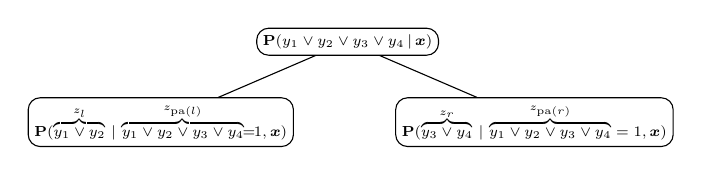
\begin{tikzpicture}[scale = 0.75,every node/.style={scale=0.75},
		regnode/.style={circle,draw,minimum width=1.5ex,inner sep=0pt},
		leaf/.style={circle,fill=black,draw,minimum width=1.5ex,inner sep=0pt},
		pleaf/.style={rectangle,rounded corners=1ex,draw,font=\scriptsize,inner sep=3pt},
		pnode/.style={rectangle,rounded corners=1ex,draw,font=\scriptsize,inner sep=3pt},
		rootnode/.style={rectangle,rounded corners=1ex,draw,font=\scriptsize,inner sep=3pt},
		activerootnode/.style={rectangle,rounded corners=1ex,draw,font=\scriptsize,inner sep=3pt,line width=1pt},
		activenode/.style={rectangle,rounded corners=1ex,draw,font=\scriptsize,inner sep=3pt,line width=1pt},
		activepleaf/.style={rectangle,rounded corners=1ex,draw,font=\scriptsize,inner sep=3pt,line width=1pt},
		level/.style={sibling distance=18em/#1, level distance=9ex}
		]
		\node (z) [rootnode] {\thickmuskip=-1.5mu $\prob(y_1\lor y_2 \lor y_3 \lor y_4 \given\bx)$}
		child {node (a) [pnode] {\thickmuskip=-1.5mu $\prob(\overbrace{y_1 \lor y_2}^{z_l}\given \overbrace{y_1 \lor y_2 \lor y_3  \lor y_4}^{z_{\mathrm{pa}(l)}}=1, \bx)$} 
			%child {node [label=below:{$y_1$}] (b) [pleaf,fill=lightgray] {\thickmuskip=-1.5mu $\prob(y_1\given y_1 \lor y_2=1, \bx)$} edge from parent node[above left]{}}
			%child {node [label=below:{$y_2$}] (g) [pleaf] {\thickmuskip=-1.5mu $\prob(y_2\given y_1 \lor y_2 = 1, \bx)$} edge from parent node[above right]{}}
			edge from parent node[above left]{}
		}
		child {node (j) [pnode] {$\prob(\overbrace{y_3 \lor y_4}^{z_r} \given \overbrace{y_1 \lor y_2 \lor y_3 \lor y_4}^{z_{\mathrm{pa}(r)}} = 1, \bx)$}
		%	child {node [label=below:{$y_3$}] (k) [pleaf] {\thickmuskip=-1.5mu $\prob(y_3\given y_3 \lor y_4 = 1, \bx)$} edge from parent node[above left]{}}
		%	child {node [label=below:{$y_4$}] (l) [pleaf] {\thickmuskip=-1.5mu $\prob(y_4\given y_3 \lor y_4 = 1,  \bx)$}
		%		{
		%			child [grow=right] {node (s) {} edge from parent[draw=none]
		%				child [grow=up] {node (t) {} edge from parent[draw=none]
		%					child [grow=up] {node (u) {} edge from parent[draw=none]}
		%				}
		%			}
		%		}
		%		edge from parent node[above right]{}
		%	}
			edge from parent node[above right]{}
		};
		\end{tikzpicture}
\caption{PLTs generalizes HSM}
\label{fig:plt-vs-hsm}
\end{figure}
%
Let us consider probabilities in sibling nodes, $l$ and $r$, as in Figure~\ref{fig:plt-vs-hsm}:
\begin{eqnarray*}
\eta_T(\bx, l) & = & \prob(z_l = 1 \given z_{\pa{l}} =1, \bx)\,,  \\
\eta_T(\bx, r) & = & \prob(z_r = 1 \given z_{\pa{r}} =1, \bx)\,.
\end{eqnarray*}
Since $\pa{l} = \pa{r}$ (as $l$ and $r$ sibling nodes, they need to have the same parent), the condition in the both probabilities above is the same. Moreover, since $z_{\pa{r}} =1$ there is at least one active label in the subtree rooted in the parent of $r$ and $l$. Since we deal with multi-class distribution, there is exactly one such label. This further implies that $z_l + z_r = 1$, and finally: 
\begin{equation}
\eta_T(\bx, l)+ \eta_T(\bx, r) = 1 \,.
\label{eqn:sibling_summation}
\end{equation}
In other words, the model in node $l$ is the complement of the model in node $r$, i.e., both sibling nodes can be collapsed to one node with one model with the left and right decision. This is then exactly the model used is binary HSM. Let us also notice that this reasoning can be nicely generalized further to $b$-ary trees.

%Summarizing the above To summarize, It uses a similar tree, but without node classifiers in leaves. To compute the probability of the $j$-th label it also uses (\ref{eqn:probabilistic_tree}), but with $\heta(\bx, j)$ being set to 1, and the sibling probabilities summing to one (\ref{eqn:sibling_summation}). 

\vspace{\sectionBefore}
\subsection{Suboptimality of the pick-one-label heuristic}
\label{sec:pick-one-label}
\vspace{\sectionAfter}

%FastText also uses HSM. 
To deal with multi-label problems HSM is often applied with the pick-one-label heuristic that randomly picks one of the labels for a given training instance. The training instance is then treated as a multi-class instance. During prediction, the heuristic returns a multi-class distribution and the most probable label only. It can be easily extended to return the top $k$ labels as in case of PLT. We will show that this approach is not consistent in general. 

%It can be easily shown that PLTs are consistent for any multi-label probability distribution $\prob$ (including the multi-class distributions).  

%This is not a case of the pick-one-label heuristic used for HSM. 
The pick-one-label heuristic maps the multi-label distribution to a multi-class distribution in the following way:\footnote{We use the same notation for the probability of the $i$-th label in the multi-class distribution as the marginal probability of the multi-label distribution, since the multi-class distribution can be also coded by vectors $\by$, but with a constraint that one and only one label is active.}
\begin{equation}
\eta'(\bx, j) = \prob'(y_j = 1 \given \bx) = \sum_{\by \in \calY} y_j \frac{\prob(\by \given \bx)}{\sum_{j'=1}^m y_{j'}}
\label{eq:heuristic}
\end{equation}
This is specific marginalization with respect to $y_j$ in which we divide the conditional probability of  $\prob(\by \given \bx)$ by the number of ones in $\by$. To see that the pick-one-label does not lead to the optimal solution let us consider the following conditional distribution for some $\bx$ given in the table below.
\begin{center}
\begin{tabular}{c c}
\toprule
labels $\by$ & probability $\prob(\by \given \bx)$ \\
\midrule
$\{1\}$ & 0.15 \\
$\{2\}$ & 0.1 \\
$\{1, 2\}$ & 0.25 \\
$\{3\}$ & 0.3 \\
$\{4\}$ & 0.2 \\
\bottomrule
\end{tabular}
\end{center}
The optimal top 1 prediction for this example is obviously label $1$, since the marginal probabilities are $\eta(\bx,1) = 0.4, \eta(\bx,2) = 0.35,  \eta(\bx,3) = 0.3, \eta(\bx,4) =0.2$. However, the pick-one-label heuristic will transform the original distribution to the following one: $\eta'(\bx,1) = 0.275, \eta'(\bx,2) = 0.225,  \eta'(\bx,3) = 0.3, \eta'(\bx,4) =0.2$. The predicted top label will be then label $3$, giving the regret of 0.1. This shows that the heuristic is consistent neither for label-wise logistic loss nor precision@k. 

%splits the probability of labels $\{1,2\}$ to half probabilities of $\{1\}$ and $\{2\}$ yielding the following marginal probabilities: $\eta(\bx,1) = 0.275, \eta(\bx,2) = 0.225,  \eta(\bx,3) = 0.3, \eta(\bx,4) =0.2$. 

In general, it is obvious that the heuristic changes the marginal probabilities of labels, unless the distribution is multi-class. 
Interestingly, if the labels are conditionally independent, i.e.,:
$$
\prob(\by \given \bx) = \prod_{j=1}^m \prob(y_i \given \bx)\,,
$$
the optimal solution in terms of precision@k will not change. To show this let us observe the following.
Let $y_i$ and $y_j$ be so that $\prob(y_i = 1 \given \bx) \ge \prob(y_j = 1 \given \bx) $. Then in the summation over all $\by$s in (\ref{eq:heuristic}), we are interested in four different subsets of $\calY$: 
$$
S_{i,j}^{u,w}  =  \{\by\in \calY: y_i = u \land y_j = w\} \quad u,w \in \{0,1\} \,.
$$
During mapping any $\by \in S^{0,0}_{i,j}$ does not play any role. For each $\by \in S^{1,1}_{i,j}$, the value of 
$$
y_t \frac{\prob(\by \given \bx)}{\sum_{t'=1}^m y_{t'}}
$$ 
is the same for both $y_i$ and $y_j$. Now, let $\by' \in S^{1,0}_{i,j}$ and $\by'' \in S^{0,1}_{i,j}$ be the same on all elements except the $i$-th and the $j$-th one. Then, because   $\prob(y_i = 1 \given \bx) \ge \prob(y_j = 1 \given \bx) $, we will have $\prob(\by' \given \bx) \ge \prob(\by'' \given \bx)$. Therefore, after mapping we will get $\eta'(\bx,i) \ge \eta'(\bx, j)$. 
Thus, for this specific situation of independent labels, the pick-one-label heuristic is consistent for precision@k.

%0.1 0.2
%0    0    0.72
%0    1    0.18
%1    0    0.08
%1    1    0.02
%
%
%0.09 0.019
%
%0.1 0.5
%0    0    0.45
%0    1    0.45
%1    0    0.05
%1    1    0.05

%0.075 0.475



\vspace{\sectionBefore}
\section{PLTs for document tagging}
\label{sec:plt-tagging}
\vspace{\sectionAfter}

In this section we focus on application of \Algo{PLT}s to document tagging. In general, \Algo{PLT}s can work with various document representations, such as sparse representations in a form of a bag-of-words and its TF-IDF variant, or dense representations being an output of a neural network. In the later case, \Algo{PLT}s play a role of the output layer of the network. 
  
%PLTs can be combined with various underlying document representations. In this section we briefly describe sample applications of PLTs to document tagging. 
%The described approaches differ mainly in the representation of a document, and therefore in the architecture of the entire model. In principle PLTs work the same in each of them, however in certain cases the application must be suited for the architecture.

In general, a document tagging system consists of two modules: text representation and tagging, as presented on the schema on Figure~\ref{pic:module-repres-module-tag}. The text representation module $f : \calW^{n} \rightarrow \R^{d}$ is a (not necessarily) parametric function whose input is a document being represented as a sequence of words of length $n$ and its output is the vector representation of a document. The dimension of the representation space is $d$. 
The input of the tagging module is the output of the text representation module. The output is the set of tags assigned to the document. Thus, the tagging system can be defined as $g: \R^{d} \rightarrow  \{ 0 , 1 \}^m$. 


%Input is given in form of document and a set of tags pairs. Documents consist of words that are taken from a dictionary which is a finite indexed set $\calW = \{ w_1, \dots , w_N \}$. A document is a sequence of words  $\bd_i = (w_{i,1}, \dots, w_{i,n_i})\in \calW^{n_i}$. Its tag set is represented  by a binary vector $\by_i = (y_{i,1}, \ldots, y_{i,m}) \in \{ 0 , 1 \}^m$ where $m$ is the number of possible tags. A set of documents is denoted by $\calD = \{ (\bw_i, \by_{i}) \}_{i=1}^n$. For sake of simplicity, we assume that $n_i = n$ for every $1\le i \le n$.
%
%Our approach consists of two modules: tagging and text representation modules. The text representation module $f : \calW^{n} \rightarrow \R^{d \times n+1}$ is a (not necessarily) parametric function whose input is a document and its output is the vector representation of both words and docs. The dimension of the representation space is $d$. In the simplest case, this text representation module can be the bag-of-words representation in which case $d=N$, and the doc vector (n+1\/th column of the image space of function $f$) is an all zero vector. A more sophisticated text representation module is the word2vec methodology which assigns a vector to each word whose dimension is typically $\le300$, and the doc representation is empty. 
%
%The tagging module's input is the output of the text presentation module, that is $g: \R^{d \times n+1} \rightarrow  \{ 0 , 1 \}^m$. 
%
%In case of Deep PLT, the text representation module simply assigns a vector $\bx_{i_j} \in \R^d$ to each word of a given document $\bd_i$, where $i_j$ is the index of the $j$\/th word of the document $i$, i.e. $f(\bd; \bx_1, \dots, \bx_N) = f(\bd) = \left[\bx_{i_1}, \dots , \bx_{i_n}, \mathbf{0}\right]$ and the document vector is zero. The labeling module is then a PLT model denoted by $g : \R^d \rightarrow  \{ 0 , 1 \}^m$ which projects the text representation to the unit vector $g( \mathbf{1}^T  f(\bd))$.
%
%DocTag2Vec is a more sophisticated model, since it makes use of document representation, however it does not make use of the text representation. The text representation module is an extended CBOW model where a document vector is added to each context that is specific to the document. Formally, the tagging module can be written as $f(\bd; \bx_1, \dots, \bx_N)=\left[\bx_{i_1}, \dots , \bx_{i_n}, \bc_i \right]$ where $\bc_i \in \R ^d$ is the representation of the document. 


\begin{figure}
	\begin{center}
		
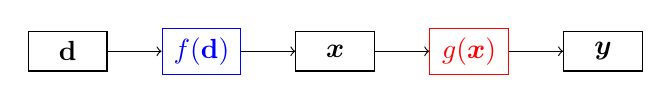
\begin{tikzpicture}[block/.style = {rectangle, draw, minimum height=0.5cm, minimum width=1cm}
]
%,yshift=0.5cm


\node (layerinput)[block]{$\mathbf{d}$};
\node (layerrepresentation)[block,right of=layerinput, xshift=.7cm, blue]{$f(\mathbf{d})$};
\node (x)[block,right of=layerrepresentation, xshift=.7cm]{$\bx$};
\node (layertagger)[block,right of=x, xshift=.7cm, red]{$g(\bx)$};
\node (layeroutput)[block,right of=layertagger, xshift=.7cm]{$\by$};

%\draw [red, thick, aligned dash] (-3.75,0.48) rectangle (3.75,-1.5);

\draw[->] ($(layerinput.north east)!0.5!(layerinput.south east)$) -- node[below] {} ($(layerrepresentation.north west)!0.5!(layerrepresentation.south west)$);
\draw[->] ($(layerrepresentation.north east)!0.5!(layerrepresentation.south east)$) -- node[above]{} ($(x.north west)!0.5!(x.south west)$);
\draw[->] ($(x.north east)!0.5!(x.south east)$) -- node[above]{} ($(layertagger.north west)!0.5!(layertagger.south west)$);
\draw[->] ($(layertagger.north east)!0.5!(layertagger.south east)$) -- node[below] {} ($(layeroutput.north west)!0.5!(layeroutput.south west)$);

\end{tikzpicture}
%\end{document}
	\end{center}
	\caption{A schema of a document tagging system.}
	\label{pic:module-repres-module-tag}
\end{figure}


%\vspace{\sectionBefore}
%\subsection{Online training of PLTs}
%\label{sec:online_PLTs}
%\vspace{\sectionAfter}
%
%PLTs can be trained by using online algorithms such as different variants of stochastic gradient descent~\citep{Bottou_2010}. This is because each node can be trained in isolation (there is no dependence between node classifiers). Since the goal is to train a model for estimating probabilities $\heta_T(\bx,j)$, one can use any algorithm that minimizes log and squared error loss. By appropriate assignment of training examples to nodes (as in Algorithm~\ref{alg:plt-training}) we can easily observe that the node classifiers can be updated in online manner. 
%This is important as in case of text classification problems we usually deal with data sets of a large number of examples (i.e., text documents). Moreover, a PLT can also be easily used as the last layer in a deep or shallow neural network. 
%
%%To apply PLTs to large data and neural networks an online training algorithm is necessary.
%%The online training algorithm for PLTs is given in Algorithm \ref{algo:plt-train}. 
%%Let $(\bx, \by)$ be a training example. The online update of a PLT requires finding the sum, denoted with  $N_{path}$, of the sets of nodes on $\Path{y_i}$ for all $y_i \in \mathcal{P}(\by)$. The set of neighbors of nodes in $N_{path}$ that are not in $N_{path}$ is denoted with $N_{\lnot path}$. All nodes in $N_{path}$ are updated with $(\bx, 1)$, and all the nodes in $N_{\lnot path}$ with $(\bx, 0)$. The described learning algorithm can be applied to many different underlying models for document representation. 
%%%
%\begin{algorithm}[]
%	\caption{Incremental learning of a \Algo{PLT}}
%	\label{algo:plt-train}
%	\begin{algorithmic}[1]
	\State \textbf{input:} a label tree $T$, an online learning algorithm $A_{\textrm{online}}$, and a training set $\mathcal{S}$
	\State \textbf{output:} a set of probability estimation classifiers $\mathcal{G}$
	\State $\mathcal{G} = \emptyset$
	\For{each node $t \in T$} 
	\State $\heta_T(\cdot,t) = \textsc{nc}()$  
	\State  $\mathcal{G} = \mathcal{G} \cup \heta_T(\cdot,t) $  
	\EndFor
	
	\For{each instance $(\bx, \by) \in \mathcal{S}$}
	
	\If{$|\mathcal{P}(\by) = 0$}
	\State $N_{\textrm{path}} = \emptyset$
	\State ${N}_{\lnot \textrm{path}} = \{r_T\}$
	\Else
	
	\State $N_{\textrm{leaf}} = \{\leaf{\ell_i} : \ell_i \in \mathcal{P}(\by)\}$
	\State $N_{\textrm{path}} = \bigcup\limits_{i \in {N}_{\textrm{leaf}} } \Path{i}$
	%\State ${N}_{\lnot path} = \textsc{Neighbors}({N}_{path})$ \Comment{a set of neighbor nodes of ${N}$ that are not in ${N}$}
	\State ${N}_{\lnot \textrm{path}} = \{t \in T: \exists_{t' \in N_{\textrm{path}}} \pa{t} = \pa{t'}\} \setminus N_{\textrm{path}}$

	\EndIf
	
	\For{$t \in \mathcal{N}_{\textrm{path}}$}
	$\heta_T(\cdot,t) = A_{\textrm{online}}(\heta_T, \bx, 1)$
	\EndFor
	
	\For{$t \in \mathcal{N}_{\lnot \textrm{path}}$}
	$\heta_T(\cdot,t) = A_{\textrm{online}}(\heta_T, \bx, 0)$
	\EndFor
	
	\EndFor		
	\State \textbf{return} a set of probability estimation classifiers $\mathcal{H}$. 
\end{algorithmic}

%\end{algorithm}
%

\vspace{\sectionBefore}
\subsection{PLTs with sparse input}
\label{sec:plt-sparse}
\vspace{\sectionAfter}

In the simplest case PLTs can be used on sparse representation of text. In other words, the text representation module $f$ can transform text to bag-of-words representation, in which case $d$ is equal to the size $N$ of the word dictionary. However, on average the number of non-zero features $\overline{\mathrm{nnz}}(\bx) \ll N$, and a document can be represented as a sparse vector. 
%There are two possibilities how to work with the sparse representation. When batch training is feasible, one can train the models effectively one by one, or in parallel, in a dense format, and then store them in a sparse format. However, when online training is required, it is necessary to use of feature hashing~\citep{Weinberger_et_al_2009} to make the memory requirements feasible. 

Interestingly, in the case of sparse features, the space complexity of \Algo{PLT}s can be significantly reduced. Admittedly, the number of models is the highest for binary trees and can be as high as $2m-1$ (notice that the size of a tree with $m$ leaves is upper bounded by $2m-1$). This is twice the number of models in the simplest 1-vs-all approach. Paradoxically, the space complexity can be the lowest at this upper bound. This is because the models need to use only the non-zero features of the training examples common for the sibling nodes; no other features are needed to build corresponding classifiers. To train a \Algo{PLT} efficiently in this situation, one needs to store the weights of the node models in hash tables and use an appropriate variant of stochastic gradient descent, in which weights of the non-zero features are updated only. If the space complexity still exceeds the available memory, one can always use feature hashing over all nodes \cite{Weinberger_et_al_2009}.


\vspace{\sectionBefore}
\subsection{PLTs with word embeddings}
\label{sec:plt-word_embeddings}
\vspace{\sectionAfter}

Instead of the sparse representation one can also use a dense representation being a result of a deep or shallow neural network. This idea is presented on Figure~\ref{pic:model-embedding}.

One possibility is to use pretrained word embeddings, like those from word2vec~\citep{Mikolov_et_al_2013} or glove~\citep{Pennigton_et_al_2014} obtained on large text corpuses. The document representation can be then created from these word embeddings in many ways, for example, as an average or as the maximum or minimum value of each element of the embeddings~\citep{De_Boom_et_al_2016}.

Alternatively, one can train the word embeddings simultaneously with the tagger module, similarly as in FastText~\citep{Joulin_et_al_2016}. Depending on the application and the size of the text corpus this might be either inferior or superior to the former approach. Another option is to initiate the network with the pretrained embeddings and then update all the parameters of both the tagging and text representation module. 
%but such approach leads to serious lengthening of the training time \cite{!!} and often to worse results\cite{!!}. This is not surprising since the pretrained word embeddings represent knowledge transfered from larger text corpora then the tagging datasets.

\begin{figure}
	\begin{center}
		
%\usepackage{tikz}
%\usetikzlibrary{positioning,calc}
%  \tikzset{}
%  }

\makeatletter
\def\pgf@dec@dashon{5pt}
\def\pgf@dec@dashoff{5pt}
\pgfkeys{/pgf/decoration/.cd,
	dash on/.store in=\pgf@dec@dashon,
	dash off/.store in=\pgf@dec@dashoff
}
\pgfdeclaredecoration{aligned dash}{start}{
	\state{start}[width=0pt, next state=pre-corner,persistent precomputation={
		\pgfextract@process\pgffirstpoint{\pgfpointdecoratedinputsegmentfirst}%
		\pgfextract@process\pgfsecondpoint{\pgfpointdecoratedinputsegmentlast}%
		\pgfmathsetlengthmacro\pgf@dec@dashon{\pgf@dec@dashon}%
		\pgfmathsetlengthmacro\pgf@dec@dashoff{\pgf@dec@dashoff}%
		\pgfmathsetlengthmacro\pgf@dec@halfdash{\pgf@dec@dashon/2}%
	}]{}
	\state{pre-corner}[width=\pgfdecoratedinputsegmentlength, next state=post-corner, persistent precomputation={
		%
		\pgfmathparse{int(ceil((\pgfdecoratedinputsegmentlength-\pgf@dec@dashon-\pgf@dec@dashoff)/(\pgf@dec@dashon+\pgf@dec@dashoff)))}%
		\let\pgf@n=\pgfmathresult
		\pgfmathsetlengthmacro\pgf@b%
		{\pgfdecoratedinputsegmentlength/(\pgf@n+1)-\pgf@dec@dashon}%
		\ifdim\pgf@b<\pgf@dec@dashoff\relax%
		\pgfmathparse{int(\pgf@n-1)}\let\pgf@n=\pgfmathresult%
		\pgfmathsetlengthmacro\pgf@b%
		{\pgfdecoratedinputsegmentlength/(\pgf@n+1)-\pgf@dec@dashon}%
		\fi%
		\pgfmathsetlengthmacro\pgf@b{\pgf@b+\pgf@dec@dashon}%
	}]{%
	\pgfmathloop
	\ifnum\pgfmathcounter>\pgf@n%
	\else%
	\pgfpathmoveto{\pgfpoint{\pgf@b*\pgfmathcounter-\pgf@dec@halfdash}{0pt}}%
	\pgfpathlineto{\pgfpoint{\pgf@b*\pgfmathcounter+\pgf@dec@halfdash}{0pt}}%
	\repeatpgfmathloop%
	\pgfpathmoveto%
	{\pgfpoint{\pgfdecoratedinputsegmentlength-\pgf@dec@halfdash}{0pt}}%
	\pgfpathlineto%
	{\pgfpointdecoratedinputsegmentlast}
}
\state{post-corner}[width=0pt, next state=pre-corner]{
	\pgfpathlineto{\pgfpoint{\pgf@dec@halfdash}{0pt}}%
}
\state{final}{
	\pgftransformreset%
	\pgfpathlineto{\pgfpointlineatdistance{\pgf@dec@halfdash}{\pgffirstpoint}{\pgfsecondpoint}}%
}
}
\tikzset{aligned dash/.style={
		decoration={aligned dash, #1}, decorate
	}}
	
	\begin{tikzpicture}[layer/.style = {rectangle, draw, minimum height=0.5cm, minimum width=7cm},
	xinput/.style = {rectangle, draw, minimum height=0.5cm, minimum width=1cm},
	dotsinput/.style = {rectangle, minimum height=0.5cm, minimum width=1cm},
	]
	%,yshift=0.5cm
	
	
	\node (layerembedding)[layer]{word embeddings};
	\node (layeragregation)[layer,above of=layerembedding]{$\bx$};
	\node (layertagger)[layer,above of=layeragregation]{PLT};
	\node (layeroutput)[layer,above of=layertagger]{output};
	
	\node (x1)[xinput,below of=layerembedding, xshift=-3cm]{$w_1$};
	\node (x2)[xinput,below of=layerembedding, xshift=-1.5cm]{$w_2$};
	\node (xdots)[dotsinput,below of=layerembedding, xshift=0cm]{\ldots};
	\node (x3)[xinput,below of=layerembedding, xshift=1.5cm]{$w_{n-1}$};
	\node (x4)[xinput,below of=layerembedding, xshift=3cm]{$w_{n}$};
	
	\draw [red, thick, aligned dash] (-3.75,3.5) rectangle (3.75,1.52);
	\draw [blue, thick, aligned dash] (-3.75,1.48) rectangle (3.75,-1.5);
	
	\draw[->] ($(layerembedding.north west)!0.5!(layerembedding.north east)$) -- node[below] {} ($(layeragregation.south west)!0.5!(layeragregation.south east)$);
	\draw[->] ($(layeragregation.north west)!0.5!(layeragregation.north east)$) -- node[below] {} ($(layertagger.south west)!0.5!(layertagger.south east)$);
	\draw[->] ($(layertagger.north west)!0.5!(layertagger.north east)$) -- node[below] {} ($(layeroutput.south west)!0.5!(layeroutput.south east)$);
	
	
	\draw[->] ($(x1.north west)!0.50!(x1.north east)$) -- node[below] {} ($(layerembedding.south west)!0.07142857142!(layerembedding.south east)$);
	
	
	\draw[->] ($(x2.north west)!0.50!(x2.north east)$) -- node[below] {} ($(layerembedding.south west)!0.28571428571!(layerembedding.south east)$);
	
	
	\draw[->] ($(x3.north west)!0.50!(x3.north east)$) -- node[below] {} ($(layerembedding.south west)!0.71428571428!(layerembedding.south east)$);
	
	
	\draw[->] ($(x4.north west)!0.50!(x4.north east)$) -- node[below] {} ($(layerembedding.south west)!0.92857142857!(layerembedding.south east)$);
	% more arrows here
	\end{tikzpicture}
	
	
%%\usepackage{tikz}
%%\usetikzlibrary{positioning,calc}
%%  \tikzset{}
%%  }
%
%\makeatletter
%\def\pgf@dec@dashon{5pt}
%\def\pgf@dec@dashoff{5pt}
%\pgfkeys{/pgf/decoration/.cd,
%	dash on/.store in=\pgf@dec@dashon,
%	dash off/.store in=\pgf@dec@dashoff
%}
%\pgfdeclaredecoration{aligned dash}{start}{
%	\state{start}[width=0pt, next state=pre-corner,persistent precomputation={
%		\pgfextract@process\pgffirstpoint{\pgfpointdecoratedinputsegmentfirst}%
%		\pgfextract@process\pgfsecondpoint{\pgfpointdecoratedinputsegmentlast}%
%		\pgfmathsetlengthmacro\pgf@dec@dashon{\pgf@dec@dashon}%
%		\pgfmathsetlengthmacro\pgf@dec@dashoff{\pgf@dec@dashoff}%
%		\pgfmathsetlengthmacro\pgf@dec@halfdash{\pgf@dec@dashon/2}%
%	}]{}
%	\state{pre-corner}[width=\pgfdecoratedinputsegmentlength, next state=post-corner, persistent precomputation={
%		%
%		\pgfmathparse{int(ceil((\pgfdecoratedinputsegmentlength-\pgf@dec@dashon-\pgf@dec@dashoff)/(\pgf@dec@dashon+\pgf@dec@dashoff)))}%
%		\let\pgf@n=\pgfmathresult
%		\pgfmathsetlengthmacro\pgf@b%
%		{\pgfdecoratedinputsegmentlength/(\pgf@n+1)-\pgf@dec@dashon}%
%		\ifdim\pgf@b<\pgf@dec@dashoff\relax%
%		\pgfmathparse{int(\pgf@n-1)}\let\pgf@n=\pgfmathresult%
%		\pgfmathsetlengthmacro\pgf@b%
%		{\pgfdecoratedinputsegmentlength/(\pgf@n+1)-\pgf@dec@dashon}%
%		\fi%
%		\pgfmathsetlengthmacro\pgf@b{\pgf@b+\pgf@dec@dashon}%
%	}]{%
%	\pgfmathloop
%	\ifnum\pgfmathcounter>\pgf@n%
%	\else%
%	\pgfpathmoveto{\pgfpoint{\pgf@b*\pgfmathcounter-\pgf@dec@halfdash}{0pt}}%
%	\pgfpathlineto{\pgfpoint{\pgf@b*\pgfmathcounter+\pgf@dec@halfdash}{0pt}}%
%	\repeatpgfmathloop%
%	\pgfpathmoveto%
%	{\pgfpoint{\pgfdecoratedinputsegmentlength-\pgf@dec@halfdash}{0pt}}%
%	\pgfpathlineto%
%	{\pgfpointdecoratedinputsegmentlast}
%}
%\state{post-corner}[width=0pt, next state=pre-corner]{
%	\pgfpathlineto{\pgfpoint{\pgf@dec@halfdash}{0pt}}%
%}
%\state{final}{
%	\pgftransformreset%
%	\pgfpathlineto{\pgfpointlineatdistance{\pgf@dec@halfdash}{\pgffirstpoint}{\pgfsecondpoint}}%
%}
%}
%\tikzset{aligned dash/.style={
%		decoration={aligned dash, #1}, decorate
%	}}
%	
%\begin{tikzpicture}[layer/.style = {rectangle, draw, minimum height=0.5cm, minimum width=7cm},
%xinput/.style = {rectangle, draw, minimum height=0.5cm, minimum width=1cm},
%]
%        %,yshift=0.5cm
%        
%        
%    \node (layerembedding)[layer]{word embeddings};
%    \node (layertagger)[layer,above of=layerembedding]{PLT};
%    \node (layeroutput)[layer,above of=layertagger]{output};
%    
%    \node (x1)[xinput,below of=layerembedding, xshift=-3cm]{$x_1$};
%    \node (x2)[xinput,below of=layerembedding, xshift=-1.5cm]{$x_2$};
%    \node (x3)[xinput,below of=layerembedding, xshift=1.5cm]{$x_{d-1}$};
%    \node (x4)[xinput,below of=layerembedding, xshift=3cm]{$x_{d}$};
%    
%    \draw [blue, thick, aligned dash] (-3.75,2.5) rectangle (3.75,0.52);
%    \draw [red, thick, aligned dash] (-3.75,0.48) rectangle (3.75,-1.5);
%    
%    \draw[->] ($(layerembedding.north west)!0.5!(layerembedding.north east)$) -- node[below] {} ($(layertagger.south west)!0.5!(layertagger.south east)$);
%    \draw[->] ($(layertagger.north west)!0.5!(layertagger.north east)$) -- node[below] {} ($(layeroutput.south west)!0.5!(layeroutput.south east)$);
%    
%    
%    \draw[->] ($(x1.north west)!0.50!(x1.north east)$) -- node[below] {} ($(layerembedding.south west)!0.07142857142!(layerembedding.south east)$);
%    
%    
%    \draw[->] ($(x2.north west)!0.50!(x2.north east)$) -- node[below] {} ($(layerembedding.south west)!0.28571428571!(layerembedding.south east)$);
%    
%    
%    \draw[->] ($(x3.north west)!0.50!(x3.north east)$) -- node[below] {} ($(layerembedding.south west)!0.71428571428!(layerembedding.south east)$);
%    
%    
%    \draw[->] ($(x4.north west)!0.50!(x4.north east)$) -- node[below] {} ($(layerembedding.south west)!0.92857142857!(layerembedding.south east)$);
%    % more arrows here
%\end{tikzpicture}
%%\end{document}
	\end{center}
	\caption{PLT with word embedding.}
	\label{pic:model-embedding}
\end{figure}


%\vspace{\sectionBefore}
%\subsection{PLTs with recurrent neural network}
%\label{sec:sparse_input}
%\vspace{\sectionAfter}

\vspace{\sectionBefore}
\subsection{PLTs with deep networks}
\label{sec:plt-deep}
\vspace{\sectionAfter}

To improve the document representation, instead of a simple aggregation over words, one can feed the embeddings of consecutive words into a more advance deep architecture, such as LSTM ~\citep{Hochreiter_Schmidhuber_1997} or the text-based convolution neural network~\cite{Liu_et_al_2017}. \Algo{PLT}s can be used with such architecture as the output layer. However, the speed advantage of this tree architecture might not be so visible in case of GPU-based training, as matrix multiplication can be efficiently performed on GPUs. 

\vspace{\sectionBefore}
\subsection{Ensemble of PLTs}
\label{sec:plt-ensemble}
\vspace{\sectionAfter}

Simultaneously to improving the document representation, one can extend the tagger module with additional PLT instances.
Depending on the tree structure, the PLT's accuracy of prediction for specific labels may vary.
Thus the aggregation of predictions from an ensemble of PLTs with random tree structures leads to improvement of the overall predictive performance.
Additionally, bootstrap aggregation can be applied to increase trees' variance further.

Document representation can be updated using %ensemble of PLTs as well as single PLT by averaging the gradients
the average of gradients obtained from separate trees, which besides may lead to a reduction of overfitting.

%Taking into account fact, that the distribution of labels in the extream classification problems follows the Pareto distribution, it is expected to achive improvment.


%%%%%%%%%%%%%%%%%%%%%%%%%%%%%%%%%%%%%%%%%%%%%%%%%%%%%%%%%%%%%%%%%%%%%%%%%%%%%%%%%%%%%%%%%%%%%%%%%%%%%%%%%%%%%%%%%%%
%%%%%%%%%%%%%%%%%%%%%%%%%%%%%%%%%%%%%%%%%%%%%%%%%%%%%%%%%%%%%%%%%%%%%%%%%%%%%%%%%%%%%%%%%%%%%%%%%%%%%%%%%%%%%%%%%%%
%%%%%%%%%%%%%%%%%%%%%%%%%%%%%%%%%%%%%%%%%%%%%%%%%%%%%%%%%%%%%%%%%%%%%%%%%%%%%%%%%%%%%%%%%%%%%%%%%%%%%%%%%%%%%%%%%%%
\vspace{\sectionBefore}
\section{Empirical results}
\label{sec:empirical_results}
\vspace{\sectionAfter}

The experimental studies presented in this section are aimed at showing advantages of the PLT approach. In the first set of experiments, we test \Algo{HSM} and \Algo{PLT} in situations where label dependency is present in the data. To this end, we work with synthetic data. In the second set of experiments, we shall compare the performance of PLT with various state-of-the-art algorithm on XMLC benchmark datasets.

%We evaluate the modesl in terms of Prec@$\{1,3,5\}$.

\subsection{Comparison of PLTs and HSM on synthetic data}
\label{sec:empirical-synthetic}

\begin{table}[]
	\centering
	\caption{Precision@1 of PLT and HSM on synthetic data. The number of passes gives the number of epochs of training. The values of precision@1 are averages of 10 random runs.}
	\label{tab:synthetic1}
\begin{tabular}{l|rr|rr|rr}
	\toprule
	 & \multicolumn{2}{c|}{dependent}                     & \multicolumn{2}{c|}{independent}                   & \multicolumn{2}{c}{multiclass}                    \\
	 passes & \multicolumn{1}{c}{PLT} & \multicolumn{1}{c|}{HSM} & \multicolumn{1}{c}{PLT} & \multicolumn{1}{c|}{HSM} & \multicolumn{1}{c}{PLT} & \multicolumn{1}{c}{HSM} \\
	\midrule
	1      & 73.17 & 72.04 & 61.87    & 53.64 & 34.31  & 34.31  \\
	10     & 85.51 & 84.16 & 63.36    & 58.00 & 38.67  & 38.67  \\
	100    & 89.09 & 85.48 & 62.23    & 60.45 & 36.71  & 36.71  \\
	1000   & 87.12 & 84.76 & 62.69    & 61.98 & 34.26  & 34.26 \\
	\bottomrule
\end{tabular}
\vspace{-0.4cm}
\end{table}


In the first set of experiments, we validate our theoretical results presented in Section 4, namely, the \Algo{HSM} is not amenable to model the conditional probabilities in general, when they are not conditionally independent. In this learning scenario, \Algo{HSM} can be outperformed in terms of Precision@K by models, like \Algo{PLT}, which has vanishing regret for conditional estimates, and so, for Precision@K (see Subsection 4.1). To validate this claim empirically, we compared the performance of \Algo{PLT} and \Algo{HSM} on synthetic datasets of three types: multi-label data with independent labels, multi-label data with conditionally dependent labels and multi-class data. 

% The independent multi-label data is generated from a multi-label BR model with randomly generated input. Each component of the input feature vector $\bx$ is generated i.i.d from uniform distribution on $[-0.5, 0.5]$ as well as the parameters of the BR model. More concretely, the score for instance $\bx$ is computed as $a_i =\bx^{T} \bw_i$ for the $i$-th label where $w_i$ is the corresponding parameter vector of BR. The score is then transformed to a probability as $p_i = \frac{1}{(1 + \exp(-a_i))}$, and the $i$-th label was drawn from Bernoulli distribution with parameter $p_i$. The multi-class data was generated based on this model as independent multi-label data, but the label was drawn from multinomial distribution with parameters $(p_1, \dots , p_m)$.

All models we used to generate synthetic data are based on $m$ linear functions $[f_1(\cdot), f_2(\cdot), \ldots, f_m(\cdot)]$ with parameters $[\boldsymbol{w}_1, \boldsymbol{w}_2, \ldots, \boldsymbol{w}_m]$. Feature vectors $\bx$ were uniformly drawn from a $d$-dimensional ball of radius $1$. Parameter vectors $\boldsymbol{w}_i$ were drawn uniformly from a $d$-dimensional sphere. All the function parameters are represented as a $m \times d$-dimensional matrix $\boldsymbol{W}$. For each sampled $\bx$ $\boldsymbol{f}(\bx) = \boldsymbol{W}\bx$  is a $m$-dimensional scores vector.

To generate the multi-class data we employ a multinomial logistic model. We take the $\boldsymbol{f}(\bx)$ and transform them with a softmax function to probabilities vector $\boldsymbol{p}(\bx)$, and we draw the positive label from this multinomial distribution.
To generate the independent multi-label data we use a binary logistic model for each of $m$ labels. We transform the score for each label $i$, $f_i(\bx)$, using a sigmoid function we get probabilities $p_i(\bx)$. For each label $i$ we draw whether it is positive with probability $p_i(\bx)$. In order to generate the conditionally dependent multi-label data we introduce transform scores using 
\begin{equation*}
\by = \assert{\boldsymbol{M} (\boldsymbol{f} +  \epsilon ) >  0  },
\end{equation*}
where $\epsilon$ a random noise and $\boldsymbol{M}$ a mixing matrix, introducing dependencies between labels. The noise $\epsilon$ is a $m$-dimensional vector drawn from $N(0, 0.25)$, and the $m \times m$ mixing matrix $\boldsymbol{m}$ i.i.d. from $[-1, 1]$. The $\assert{\cdot}$ is applied to each element separately.


%To validate the theoretical results we perform a comparison of PLTs and HSM on synthetic datasets of three types: multi-label with conditionally dependent labels, multi-label with independent labels, and multi-class. The empirical results are given in Table \ref{tab:synthetic1}. The methods used to generate the data are given below.
%
%The independent multi-label data was generated from a multi-label OvR model. Example features $\bx$ were generated by uniformly drawing from $[-0.5, 0.5]^d$. The OvR weights $W$ were drawn uniformly from  $[-0.5, 0.5]^{d \times m}$.
%%, where $s$ stands for a shift used to control the average probability of a positive label. 
%The score $a =\bx w_i$ of $i$-th label was then transformed to a probability $p_i(a) = \frac{1}{(1 + exp(-a))}$, and the $i$-th label was drawn with the probability $p_i$.
%
%% The conditionally dependent multi-label data was generated from the PCC \cite{!} model. Example features were drawn as in the previous paragraph. The PCC model weights were drawn from  $[-0.5, 0.5]^{(d + m) \times m}$.
%% %, also with the use of a shift $s$. 
%% The score of $i$-th label was computed based on it's features and all the previous labels $j$ as $d+j$-th features, set to -$q$ or $q$ depending on the results of the draws with labels probabilities. The value of $q$, usually set to $0.5$, is related to the degree of dependence between labels.
%
%
%The conditionally dependent multi-label data was generated according to the following model:
%\begin{equation*}
%\boldsymbol{f} = \boldsymbol{A }\bx + \epsilon 
%\end{equation*}
%\begin{equation*}
%\by = \assert{\boldsymbol{M} \boldsymbol{f} >  0  },
%\end{equation*}
%
%\noindent
%where $\boldsymbol{f} = (f_1, f_2, \ldots, f_m)$ represent $m$ latent variables, $\boldsymbol{M}$ a mixing matrix, and $\epsilon$ a noise introducing label dependencies. The two-dimensional feature vector $\bx$ was drawn uniformly from a unit disc, the linear coefficients $A$ uniformly from two-dimensional unit sphere. The noise $\epsilon$ is a $m$-dimensional vector drawn from $N(0, 0.25)$, and the $m \times m$ mixing matrix $\boldsymbol{m}$ i.i.d. from $[-1, 1]$. To make the labels dependent $\boldsymbol{M} \neq \boldsymbol{I}$.
%
%The multi-class data was generated based on the same model as independent multi-label data, OvR, but we selected the label with the highest probability, instead of drawing $m$ times. 
%
%\textbf{TODO: this table will contain some other results}



The results are shown in Table \ref{tab:synthetic1}. The train/test data was generated from our generative models in each repetition. The weights of \Algo{PLT} and \Algo{HSM} learners were initialized by the same random values for a fair comparison. Consequently, the performance of \Algo{HSM} and \Algo{PLT} on multi-class data match to each other, as one would expect this. On data with conditionally independent labels, the performance of \Algo{HSM} and \Algo{PLT} is on-par after $1000$ iteration. The difference in convergence speed can be explained by the fact that \Algo{HSM} updates the model by picking one positive label at once, wheres \Algo{PLT}  carries out the updates for all positive label simultaneously. On data with dependent label, \Algo{PLT} outperforms \Algo{HSM}. This coincide with our theoretical finding regarding the non-vanishing regret of \Algo{HSM}. 





\subsection{Benchmark data}

We also carried out experiments on commonly used benchmark datasets taken from XMLC repository~\footnote{http://manikvarma.org/downloads/XC/XMLRepository.html} and Yahoo news multi-label corpus~\footnote{https://yahooresearch.tumblr.com/post/164789421126/introducing-the-yahoo-news-ranked-multi-label}. Every datasets we used consists of text data, so we decided to use two representations of them when it is available: feature vectors taken from XMLC repository, and word embeddings described in Subsection \ref{sec:word_embeddings}. In case of Yahoo! news dataset we used bag of words representation.


\begin{table}[ht!]
\vspace{-.2cm}
        \caption{Precision@K scores with $K=\{ 1,3,5\}$ of \Algo{HSM}, \Algo{LOM} and \Algo{PLT} algorithms. }
        \label{tab:hsm_vs_plt}
        \begin{center}
                \begin{small}
                        \vspace{-0.1cm}
                        \begin{tabular}{l@{\hskip 0pt} | r@{\hskip 0pt} | r@{\hskip 0pt} | r@{\hskip 0pt} | r@{\hskip 0pt} }
                                \toprule
	& \multicolumn{2}{|c|}{\Algo{XMLC}} & \multicolumn{2}{|c}{\Algo{Word embeddings}} \\ \midrule
	& \multicolumn{1}{|c|}{\Algo{HSM}} & \multicolumn{1}{|c}{\Algo{PLT}} & \multicolumn{1}{|c|}{\Algo{HSM}} & \multicolumn{1}{|c}{\Algo{PLT}} \\ \midrule
	Yahoo! & \data{}{}{} & \data{70.06}{58.04}{46.05} & \data{67.80}{54.88}{43.78} & \data{71.79}{58.82}{46.38} \\ \midrule
	RCV1 & \data{87.73}{69.98}{50.17} & \data{90.47}{72.54}{51.84} & \data{93.94}{76.75}{53.61} & \data{95.41}{77.49}{53.91} \\ \midrule
	Wiki30k & \data{70.20}{60.11}{53.17} & \data{84.34}{72.34}{62.72} & \data{83.02}{69.66}{59.50} & \data{85.11}{73.12}{62.67} \\ \midrule
	Amazon12(13?)k & \data{86.69}{72.00}{57.97} & \data{91.46}{76.00}{61.40} & \data{90.18}{72.53}{56.20} & \data{92.98}{75.75}{59.53} \\ \midrule
	EUR-Lex & \data{}{}{} & \data{74.55}{60.60}{50.05} & \data{66.39}{54.05}{44.73} & \data{73.19}{57.79}{46.98} \\ \midrule
	Delicious-200K & \data{41.58}{33.24}{28.04} & \data{45.27}{38.95}{35.59} & \data{42.17}{37.94}{35.77} & \data{46.98}{40.99}{38.04} \\ \midrule
	WikiLSHTC-325K & \data{36.90}{22.30}{16.60} & \data{41.63}{26.78}{20.39} & \data{41.28}{24.68}{18.08} & \data{41.78}{24.963}{18.529} \\ \midrule
    Amazon-670K & \data{33.64}{28.58}{25.01} & \data{36.85}{32.48}{29.15} & \data{25.04}{21.06}{18.28} & \data{26.18}{22.76}{20.29} \\
								\bottomrule
                        \end{tabular}
                \end{small}
        \end{center}
	\vspace{-0.4cm}
\end{table}


We compared the performance of \Algo{HSM} and \Algo{PLT}. We tuned the hyper-parameters of the models by using grid search. The range of the hyper-parameters is reported in Appendix. The results are shown in Table \ref{tab:hsm_vs_plt}. \Algo{PLT} clearly outperforms \Algo{HSM} in all cases by a very significant margin on both text representations. The running time of these two algorithm is 


\begin{table*}[ht!]
\vspace{-.2cm}
        \caption{Precision@K scores with $K=\{ 1,3,5\}$ of \Algo{FastXML}, \Algo{SLEEC}, \Algo{HSM}, \Algo{LOM} and \Algo{PLT} algorithms. The highest Precision@K values are in bold for every dataset.}
        \label{tab:datasets-differences-table}
        \begin{center}
                \begin{small}
                        \vspace{-0.1cm}
                        \begin{tabular}{l@{\hskip 0pt} | l@{\hskip 0pt}| r@{\hskip 0pt} | r@{\hskip 0pt} | r@{\hskip 0pt} | r@{\hskip 0pt} | r@{\hskip 0pt} | r@{\hskip 0pt} | r@{\hskip 0pt}  }
                                \toprule
& & \multicolumn{1}{|c|}{\Algo{FastXML}} & \multicolumn{1}{|c|}{\Algo{SLEEC}} & \multicolumn{1}{|c|}{\Algo{HSM}} & \multicolumn{1}{|c|}{\Algo{LOM}} & \multicolumn{1}{|c|}{\Algo{PLT}} & \multicolumn{1}{|c|}{\Algo{PLT+ens}} & \multicolumn{1}{|c}{\Algo{CNN}} \\
                                \midrule
RCV1 & \data{P@1}{P@3}{P@5} & \data{94.62}{78.40}{54.82} & \data{95.35}{79.51}{55.06} & \data{93.94}{76.75}{53.61} & \data{94.46}{77.52}{53.76} & \data{95.41}{77.49}{53.91} & \data{95.77}{\textbf{90.99}}{\textbf{82.53}} & \data{\textbf{96.83}}{81.44}{56.57} \\ \midrule
Yahoo & \data{P@1}{P@3}{P@5} & \data{}{}{} & \data{}{}{} & \data{67.80}{54.88}{43.78} & \data{67.73}{56.27}{44.55} & \data{71.79}{58.82}{46.38} & \data{\textbf{74.08}}{\textbf{69.63}}{\textbf{64.05}} & \data{71.71}{58.40}{45.62} \\ \midrule
EUR-Lex & \data{P@1}{P@3}{P@5} & \data{68.12}{57.93}{48.97} & \data{\textbf{78.21}}{64.33}{52.47} & \data{68.69}{56.52}{47.20} & \data{66.39}{54.05}{44.73} & \data{73.19}{57.79}{46.98} & \data{75.08}{\textbf{70.06}}{\textbf{63.38}} & \data{72.16}{57.32}{46.49} \\ \midrule
Wiki-30K & \data{P@1}{P@3}{P@5} & \data{83.26}{68.74}{58.84} & \data{\textbf{85.96}}{73.13}{62.73} & \data{83.02}{69.66}{59.50} & \data{81.44}{67.67}{57.85} & \data{85.11}{73.12}{62.67} & \data{85.21}{\textbf{81.29}}{\textbf{75.22}} & \data{82.78}{66.34}{56.23}\\ \midrule
Amazon-13(12?)K & \data{P@1}{P@3}{P@5} & \data{94.58}{78.69}{62.26} & \data{93.61}{79.13}{63.54} & \data{90.18}{72.53}{56.20} & \data{90.37}{73.62}{57.18} & \data{92.98}{75.75}{59.53} & \data{93.42}{\textbf{88.75}}{\textbf{80.39}} & \data{\textbf{95.13}}{79.52}{63.46} \\ \midrule
Amazon-670K & \data{P@1}{P@3}{P@5} & \data{\textbf{35.59}}{\textbf{31.87}}{\textbf{28.96}} & \data{34.54}{30.89}{28.25} & \data{25.04}{21.06}{18.28} & \data{25.67}{20.96}{18.72} & \data{26.18}{22.76}{20.29} & \data{25.66}{24.15}{22.73} & \data{?}{?}{?} \\ \midrule
Delicious-200K & \data{P@1}{P@3}{P@5} & \data{43.07}{38.66}{36.19} & \data{\textbf{47.85}}{42.21}{39.43} & \data{42.17}{37.94}{35.77} & \data{42.68}{38.24}{35.87} & \data{46.98}{40.99}{38.04} & \data{47.27}{\textbf{44.80}}{\textbf{42.28}} & \data{-}{-}{-} \\ \midrule
WikiLSHTC-325K & \data{P@1}{P@3}{P@5} & \data{49.75}{33.10}{24.45} & \data{\textbf{54.83}}{33.42}{23.85} & \data{41.28}{24.68}{18.08} & \data{50.16}{31.95}{23.59} & \data{41.78}{24.963}{18.529} & \data{40.92}{\textbf{34.19}}{\textbf{27.35}} & \data{-}{-}{-} \\
%Datasets & \data{P@1}{P@3}{P@5} & \data{}{}{} & \data{}{}{} & \data{}{}{} & \data{}{}{} & \data{}{}{} & \data{}{}{} & \data{}{}{} \\ \midrule
                                \bottomrule
                        \end{tabular}
                \end{small}
        \end{center}
	\vspace{-0.4cm}
\end{table*}


\begin{table*}[ht!]
\vspace{-.2cm}
        \caption{Training and testing time of \Algo{FastXML}, \Algo{SLEEC}, \Algo{HSM}, \Algo{LOM} and \Algo{PLT} algorithms in minutes.}
        \label{tab:datasets-differences-table}
        \begin{center}
                \begin{small}
                        %\vspace{-0.1cm}
                        \begin{tabular}{l@{\hskip 0pt} | l@{\hskip 0pt}| r@{\hskip 0pt} | r@{\hskip 0pt} | r@{\hskip 0pt} | r@{\hskip 0pt} | r@{\hskip 0pt} | r@{\hskip 0pt} | r@{\hskip 0pt}  }
                                \toprule
& & \multicolumn{1}{|c|}{\Algo{FastXML}} & \multicolumn{1}{|c|}{\Algo{SLEEC}} & \multicolumn{1}{|c|}{\Algo{HSM}} & \multicolumn{1}{|c|}{\Algo{LOM}} & \multicolumn{1}{|c|}{\Algo{PLT}} & \multicolumn{1}{|c|}{\Algo{PLT+ens}} & \multicolumn{1}{|c}{\Algo{CNN}} \\
                                \midrule
RCV1 & \datarr{train}{test} & \datarr{9.2}{10.2} & \datarr{14.8}{29.4} & \datarr{}{} & \datarr{}{} & \datarr{}{} & \datarr{}{} & \datarr{39.0}{1.48} \\ \midrule
Yahoo & \datarr{train}{test} & \datarr{}{} & \datarr{}{} & \datarr{}{} & \datarr{}{} & \datarr{}{} & \datarr{}{} & \datarr{?}{?} \\ \midrule
EUR-Lex & \datarr{train}{test} & \datarr{12.6}{0.9} & \datarr{75.95}{0.26} & \datarr{}{} & \datarr{}{} & \datarr{}{} & \datarr{}{} & \datarr{17.0}{0.7} \\ \midrule
Wiki-30K & \datarr{train}{test} & \datarr{34.1}{0.4} & \datarr{44.1}{0.01?} & \datarr{}{} & \datarr{}{} & \datarr{}{} & \datarr{}{} & \datarr{88.0}{0.15} \\ \midrule
Amazon-13(12?)K & \datarr{train}{test} & \datarr{466}{17} & \datarr{1515}{41.77} & \datarr{}{} & \datarr{}{} & \datarr{}{} & \datarr{}{} & \datarr{800}{0.75} \\ \midrule
Amazon-670K & \datarr{train}{test} & \datarr{789}{21.6} & \datarr{1083}{47.6} & \datarr{}{} & \datarr{}{} & \datarr{}{} & \datarr{}{} & \datarr{3134}{41.3} \\ \midrule
Delicious-200K & \datarr{train}{test} & \datarr{}{} & \datarr{}{} & \datarr{}{} & \datarr{}{} & \datarr{}{} & \datarr{}{} & \datarr{-}{-} \\ \midrule
WikiLSHTC-325K & \datarr{train}{test} & \datarr{}{} & \datarr{}{} & \datarr{}{} & \datarr{}{} & \datarr{}{} & \datarr{}{} & \datarr{-}{-} \\
%Datasets & \datarr{train}{test} & \datarr{}{} & \datarr{}{} & \datarr{}{} & \datarr{}{} & \datarr{}{} & \datarr{}{} & \datarr{}{} \\ \midrule
                                \bottomrule
                        \end{tabular}
                \end{small}
        \end{center}
	\vspace{-0.4cm}
\end{table*}

We also compare the performance of \Algo{PLT} with some state-of-the-art learners on benchmark dataset. As a baseline, we used Convolutional Neural Net work (CNN) models by~\citep{Liu_et_al_2017} which deep network architecture achieves very impressive  performance on these datasets.

The results reveal some general trends. The PLT outperforms LOM and HSM consistently. The bagging significantly improves the precision at higher position. 

We would especially like to underline the fact that the PLT with word embeddings is on-par with the more complex CNN model in terms of precision for a computational cost that is an order of magnitude smaller.


\section{Conclusions}

We empirically justified that \Algo{PLT} is a better model of choice when one face with multi-label classification task.

\newpage



\bibliography{xmlc_references}
\bibliographystyle{icml2018}

\appendix

\onecolumn

\section{Regret for precision@k}
\label{app:prec@k}

Precision@k is formally defined as:
$$
\mathrm{precision}@k(\by, \bx, \bh) = \frac{1}{k} \sum_{j \in \hat \calY_k} \assert{y_j = 1},
%\label{eqn:precision-at-k}
$$
where $\hat \calY_k$ is a set of $k$ labels predicted by $\bh$ for $\bx$.
%
To be consistent with the former discussion, let us define a loss function for precision@k as $\ell_{p@k} = 1 - \mathrm{precision}@k$. The conditional risk is then:
\begin{eqnarray*}
\loss_{p@k}(\bh \given \bx) & = & \mathbb{E} \ell_{p@k}(\by,\bx, \bh) \\
& = & 1 - \sum_{\by \in \calY} \prob(\by \given \bx) \frac{1}{k} \sum_{j \in \hat \calY_k} \assert{y_j = 1} \\
& = & 1 - \frac{1}{k} \sum_{j \in \hat \calY_k} \sum_{\by \in \calY} \prob(\by \given \bx) \assert{y_j = 1} \\
& = & 1 - \frac{1}{k} \sum_{j \in \hat \calY_k} \eta(\bx,j) \,.
\end{eqnarray*}
%
The above result shows that the optimal strategy for precision$@k$ is to predict $k$ labels
with the highest conditional probabilities $\eta(\bx,j)$.





Top-k labels with respect to the true marginals
\[
M_k(\bx) = \left\{ i\in [m] : \# \left\{ j \in [m] : \eta(\bx, j) \ge \eta(\bx, i)  \right\} \le k\right\}
\]

Top-k labels with respect to the estimated marginals
\[
\hat{M}_k(\bx) = \left\{ i\in [m] : \# \left\{ j \in [m] : \hat{\eta}(\bx, j) \ge \hat{\eta}(\bx, i)  \right\} \le k\right\}
\]


Expected regret for Prec@k conditioned on $\bx$ 
\[
\mbox{Reg}_{P@k} (h, \bx) = \sum_{i \in M_k(\bx)} \eta (\bx ,i ) - \sum_{j \in [m]} h(\bx, j) \eta(\bx , j )
\]

We shall focus on multi-label classifiers in the following form:
\[
h(\bx,i) =h_{k, \hat{\eta}}(\bx,i) = \assert{\textstyle i \in \hat{M}_k(\bx) }
\]

In this case the Prec@k regret is $[0,1]$.

The error for marginal estimates is denoted by $m_i = \vert \eta (\bx ,i ) - \hat{\eta} (\bx ,i )\vert$. With this we can upper bound 
\begin{align}
\mbox{Reg}_{P@k} (h, \bx) 
  & = \sum_{i \in M_k(\bx)} \eta (\bx ,i ) - \sum_{j \in [m]} h(\bx, j) \eta(\bx , j ) \notag \\
  & \le \sum_{i \in M_k(\bx)} \hat{\eta} (\bx ,i ) + m_i - \sum_{j \in [m]} h(\bx, j) \eta(\bx , j ) \notag \\ 
  & \le \sum_{i \in \hat{M}_k(\bx)} (\hat{\eta} (\bx ,i ) + m_i )- \sum_{j \in \hat{M}_k(\bx)}  \eta(\bx , j ) \notag \\
  & = \sum_{i \in \hat{M}_k(\bx)} 2m_i \notag \\
  & \le 2k\max_{i \in [m]} m_i
\end{align}

\section{Probabilistic label trees}
\label{app:plt}

An example of a probabilistic label tree (\Algo{PLT}) for 4 labels $(y_1,y_2,y_3,y_4)$ is given in Fig.~\ref{fig:plt}. To estimate posterior probability $\eta(\bx, j) = \prob(y_j = 1 \given \bx)$, \Algo{PLT} uses a path from a root to the $j$-th leaf.
In each node $t$, we associate with a training instance $(\bx,\by)$ a label $z_t$ such that:
$$
z_t = \assert{\textstyle \sum_{j \in L(t)} y_j \ge 1} \quad \textrm{(or equivalently $z_t = \bigvee_{j \in L(t)} y_j$)}
$$
Recall that $L(t)$ is a set of all leaves of a subtree with the root in the $t$-th node. In leaf nodes the labels $z_j$, $j \in L$, correspond to original labels $y_j$.
%
\begin{figure}[h]
	\begin{center}
		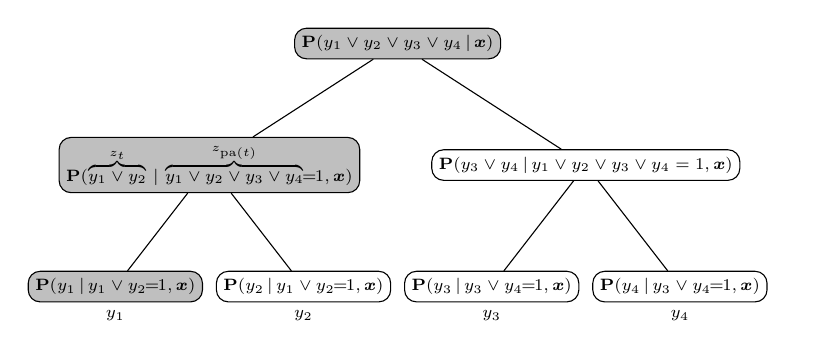
\begin{tikzpicture}[scale = 0.85,every node/.style={scale=0.85},
		regnode/.style={circle,draw,minimum width=1.5ex,inner sep=0pt},
		leaf/.style={circle,fill=black,draw,minimum width=1.5ex,inner sep=0pt},
		pleaf/.style={rectangle,rounded corners=1ex,draw,font=\scriptsize,inner sep=3pt},
		pnode/.style={rectangle,rounded corners=1ex,draw,font=\scriptsize,inner sep=3pt},
		rootnode/.style={rectangle,rounded corners=1ex,draw,font=\scriptsize,inner sep=3pt},
		activerootnode/.style={rectangle,rounded corners=1ex,draw,font=\scriptsize,inner sep=3pt,line width=1pt},
		activenode/.style={rectangle,rounded corners=1ex,draw,font=\scriptsize,inner sep=3pt,line width=1pt},
		activepleaf/.style={rectangle,rounded corners=1ex,draw,font=\scriptsize,inner sep=3pt,line width=1pt},
		level/.style={sibling distance=16em/#1, level distance=12ex}
		]
		\node (z) [rootnode,fill=lightgray] {\thickmuskip=-1.5mu $\prob(y_1\lor y_2 \lor y_3 \lor y_4 \given\bx)$}
		child {node (a) [pnode,fill=lightgray] {\thickmuskip=-1.5mu $\prob(\overbrace{y_1 \lor y_2}^{z_t}\given \overbrace{y_1 \lor y_2 \lor y_3  \lor y_4}^{z_{\mathrm{pa}(t)}}=1, \bx)$} 
			child {node [label=below:{ \scriptsize \thickmuskip=-1.5mu $y_1$}] (b) [pleaf,fill=lightgray] {\thickmuskip=-1.5mu $\prob(y_1\given y_1 \lor y_2=1, \bx)$} edge from parent node[above left]{}}
			child {node [label=below:{\scriptsize \thickmuskip=0mu $y_2$}] (g) [pleaf] {\thickmuskip=-1.5mu $\prob(y_2\given y_1 \lor y_2 = 1, \bx)$} edge from parent node[above right]{}}
			edge from parent node[above left]{}
		}
		child {node (j) [pnode] {$\prob(y_3 \lor y_4 \given y_1 \lor y_2 \lor y_3 \lor y_4 = 1, \bx)$}
			child {node [label=below:{ \scriptsize \thickmuskip=0mu $y_3$}] (k) [pleaf] {\thickmuskip=-1.5mu $\prob(y_3\given y_3 \lor y_4 = 1, \bx)$} edge from parent node[above left]{}}
			child {node [label=below:{ \scriptsize \thickmuskip=0mu $y_4$}] (l) [pleaf] {\thickmuskip=-1.5mu $\prob(y_4\given y_3 \lor y_4 = 1,  \bx)$}
				{
					child [grow=right] {node (s) {} edge from parent[draw=none]
						child [grow=up] {node (t) {} edge from parent[draw=none]
							child [grow=up] {node (u) {} edge from parent[draw=none]}
						}
					}
				}
				edge from parent node[above right]{}
			}
			edge from parent node[above right]{}
		};
		\end{tikzpicture}
\end{center}
\caption{An example of a probabilistic label tree for 4 labels $(y_1,y_2,y_3,y_4)$.}
\label{fig:plt}
\end{figure}
%

Consider the leaf node $j$ and the path from the root to this leaf node. Using the chain rule of probability, we can express $\eta(\bx, j)$ in the following way:
\begin{equation}
\eta(\bx, j) = \prod_{t \in \Path{j}} \eta_T(\bx, t)\,,
\label{eqn:probabilistic_tree_appendix}
\end{equation}
where $\eta_T(\bx, t) = \prob(z_t = 1 \given z_{\pa{t}} =1, \bx)$, for all non-root nodes $t$, and $\eta(\bx, t) = \prob(z_t = 1 \given \bx)$, if $t$ is the root node (denoted by $r(T)$). 

To see the correctness of (\ref{eqn:probabilistic_tree_appendix}) notice that $z_{t} = 1$ implies $z_{\pa{t}} = 1$. So, for non-root nodes $t$ and $\pa{t}$ we have:
\begin{eqnarray*}
\eta_T(\bx,t) \eta_T(\bx, \pa{t}) & = &  \prob(z_t = 1 \given z_{\pa{t}} =1, \bx)\prob(z_{\pa{t}} = 1 \given z_{\pa{\pa{t}}} =1, \bx)\\
& = & \frac{\prob(z_t = 1 , z_{\pa{t}} =1, \bx)}{\prob(z_{\pa{t}} =1, \bx)} \frac{\prob(z_{\pa{t}} = 1, z_{\pa{\pa{t}}} =1, \bx)}{\prob(z_{\pa{\pa{t}}} =1, \bx)} \\
& = & \frac{\prob(z_t = 1, \bx)}{\prob(z_{\pa{t}} =1, \bx)} \frac{\prob(z_{\pa{t}} = 1, \bx)}{\prob(z_{\pa{\pa{t}}} =1, \bx)} \\
& = & \frac{\prob(z_t = 1, \bx)}{\prob(z_{\pa{\pa{t}}} =1, \bx)} \,.
\end{eqnarray*}
In words, the probability associated with the parent node $\pa{t}$ cancels out and we can express $\eta_T(\bx,t) \eta_T(\bx, \pa{t})$ as the product of probabilities associated only with node $t$ and its grandparent node $\pa{\pa{t}}$. 
%
Applying the above rule consecutively to $\prod_{t \in \Path{j}} \eta_T(\bx, t)$ and recalling that for the root note $\eta_T(\bx, r(T)) = \prob(z_{r(T)} = 1 \given \bx)$, we finally get $\eta(\bx, j)$. 

Below we show that \Algo{PLT}s posses strong theoretical guarantees. We derive a relation between  estimation error minimized by the node classifiers and estimation error of posterior probabilities $\eta(\bx,j)$. This relation states that we can upperbound the latter error by the former. This also implies that for optimal node classifiers we get optimal multi-label classifier in terms of estimation of posterior probabilities.

We are interested in bounding the estimation error of posterior probabilities of labels at point $\bx$
$$
\ell(\eta(\bx),\heta(\bx)) = \frac{1}{m} \sum_{j=1}^m |\eta(\bx, j) - \heta(\bx, j)| \,,
$$
in terms of an estimation error of node classifiers
$$
\ell(\eta_T(\bx, t), \heta_T(\bx, t)) = |\eta_T(\bx, t) - \heta_T(\bx, t)  | \,.
$$

Expressing $\eta(\bx, j)$  and $\heta(\bx, j)$ by (\ref{eqn:probabilistic_tree_appendix}) and applying Lemma~2 from~\cite{Beygelzimer_et_al_2009b}, we get:
\begin{equation}
\left | \eta(\bx, j) - \heta(\bx, j) \right | \le \sum_{t \in \Path{j}} \left | \eta_T(\bx, t) - \heta_T(\bx, t) \right | \,.
\label{eqn:estimation_bound}
\end{equation}

Equation (\ref{eqn:estimation_bound}) already shows that minimization of the estimation error by node classifiers improves the overall performance of \Algo{PLT}s. We can show, however, even a more general result concerning surrogate regret bounds by referring to the theory of  strongly proper composite losses~\cite{Agarwal_2014}. 

Assume that a node classifier has a form of a real-valued function $f_t$. Moreover, there exists a strictly increasing (and therefore invertible) link function $\psi: [0,1] \rightarrow \mathbb{R}$ such that $f_t(\bx) = \psi(\heta_T(\bx,t))$. Recall that the regret of $f_t$ in terms of a loss function $\ell$ at point $\bx$ is defined as:
$$
\reg_{\ell}(f_t \given \bx) = L_{\ell}(f_t \given \bx) - L_{\ell}^*(\bx) \,,
$$
where $L_{\ell}(f_t \given \bx)$ is the expected loss  at  point $\bx$:
$$
L_{\ell}(f \given \bx) = \mathbb{E}_{y_j\given\bx} \left [ \ell  (y_j, f_t(\bx)) \right ] \,,
$$
and  $L_{\ell}^*(\bx)$ is the minimum expected loss at point $\bx$.

If a node classifier is trained by a learning algorithm that minimizes a strongly proper composite loss, e.g.,  squared, exponential, or logistic loss, like in our implementation (see in Appendix \ref{sec:training_of_node_classifiers}), then the bound (\ref{eqn:estimation_bound}) can be expressed in terms of the regret of this loss function: 
$$
\left | \eta_T(\bx, t) - \psi^{-1}(f_t)  \right | \le \sqrt{ \frac{2}{\lambda}} \sqrt{\reg_\ell(f_t \given \bx)}
$$
where $\lambda$ is a strong properness constant specific for a given loss function (for more detail, see~\cite{Agarwal_2014}). By putting the above inequality into~(\ref{eqn:estimation_bound}), we get
$$
\left | \eta(\bx, j) - \heta(\bx, j) \right | \le \! \sum_{t \in \Path{j}} \! \left | \eta_T(\bx, t) - \heta_T(\bx, t) \right | = \!  \sum_{t \in \Path{j}}  \! \left | \eta_T(\bx, t) - \psi^{-1}(f_t)  \right | \le  \! \sum_{t \in \Path{j}}  \! \sqrt{ \frac{2}{\lambda}} \sqrt{\reg_\ell(f_t \given \bx)}
$$ 


\section{Tuning of hyperparameters}
\label{sec:hyper}


A \Algo{PLT} has only one global hyperparameter which is the degree of the tree denoted by $b$. The other hyperparameters are associated with the node classifiers. To tune the stochastic gradient descent described above we varied values of $\gamma$, $\lambda$, and the number of epochs. 
%
All hyperparameters were tuned by using the open-source hyperparameter optimizer \Algo{SMAC}~\cite{Hutter_et_al_2011} with a wide range of parameters, which is reported in Table \ref{tab:hyppar}. 
%We also tuned the number of epochs which is the number of times we run through the entire dataset. 
The validation process was carried out by using a $80/20$ split of the training data for every dataset we used.

\vspace{\tableBefore}
\begin{table}[ht!]
\caption{The hyperparameters of the \Algo{PLT} method and their ranges used in hyperparameter optimization,}
\label{tab:hyppar}
\begin{center}
\begin{tabular}{|c|c|c|c|c|c|c|c|}
\hline
Hyperparameter & Validation range \\%& RCV1 & AmazonCat & Wiki10 & Delicious-200K & WikiLSHTC & Amazon \\ 
\hline
$b$ & $\{2,\dots,256\}$ \\% &  $16$          & $16$      & $32$   & $2$     & &       \\ 
$\lambda$ &  $[10 - 0.000001]$ \\%& $10^{-4}$ & $10^{-4}$   & $10^{-5}$& $10^{-5}$ & &       \\ 
$\gamma$ &  $[10 - 0.000001]$ \\%& $10^{-5}$  & $10^{-5}$   & $10^{-5}$& $10^{-6}$ & &       \\ 
Num. of epochs &  $\{ 5, \dots , 30\} $ \\
\hline
\end{tabular}
\end{center}
\end{table}
\vspace{\tableAfter}

\end{document} 



% This document was modified from the file originally made available by
% Pat Langley and Andrea Danyluk for ICML-2K. This version was created
% by Iain Murray in 2018. It was modified from a version from Dan Roy in
% 2017, which was based on a version from Lise Getoor and Tobias
% Scheffer, which was slightly modified from the 2010 version by
% Thorsten Joachims & Johannes Fuernkranz, slightly modified from the
% 2009 version by Kiri Wagstaff and Sam Roweis's 2008 version, which is
% slightly modified from Prasad Tadepalli's 2007 version which is a
% lightly changed version of the previous year's version by Andrew
% Moore, which was in turn edited from those of Kristian Kersting and
% Codrina Lauth. Alex Smola contributed to the algorithmic style files.
